%%%%%%%%%%%%%%%%%%%%%%%%%%%%%%%%%%%%%%%%%%%%%%%%%%%%%%%%%%%
% Rho-class article
%%%%%%%%%%%%%%%%%%%%%%%%%%%%%%%%%%%%%%%%%%%%%%%%%%%%%%%%%%%

\documentclass[9pt,letterpaper,twocolumn,twoside,apabib]{rho-class/rho}
\usepackage[spanish,es-nodecimaldot,es-noindentfirst,es-noshorthands]{babel}
\usepackage{longtable}
\usepackage{array}
\usepackage{pdflscape}
% \usepackage{hyperref}

% Use shortauthor abbreviations directly in citations while keeping full authors
% in the bibliography and preserving biblatex-apa's standard citation macros.

\makeatletter
\renewbibmacro*{cite:plabelyear+extradate}{%
  \iffieldundef{labelyear}{}
    {\clearfield{labelmonth}%
     \clearfield{labelday}%
     \clearfield{labelendmonth}%
     \clearfield{labelendday}%
     \clearfield{labelyeardivision}%
     \clearfield{labelendyeardivision}%
     \iffieldsequal{labelyear}{labelendyear}
       {\clearfield{labelendyear}}
       {}%
     \iffieldundef{origyear}
       {}
       {\printorigdate%
        \setunit*{\addslash}}%
     \iffieldundef{related}
       {}
       {\iffieldequalstr{relatedtype}{reprintfrom}
         {\entrydata*{\thefield{related}}{\printlabeldateextra}%
          \setunit*{\addslash}}
         {}}%
     \printlabeldateextra}}

\renewbibmacro*{cite}{%
  \printtext[bibhyperref]{%
    \iffieldequals{namehash}{\cbx@lasthash}
      {\setunit{\compcitedelim}%
       \usebibmacro{cite:plabelyear+extradate}}
      {\ifnameundef{labelname}
        {\usebibmacro{cite:noname}%
         \setunit{\printdelim{nameyeardelim}}%
         \usebibmacro{cite:plabelyear+extradate}%
         \savefield{namehash}{\cbx@lasthash}}
        {\ifnameundef{shortauthor}
          {\printnames{labelname}}
          {\cbx@apa@ifnamesaved
            {\printnames{shortauthor}}
            {\printnames[labelname]{author}%
             \addspace\printnames[sabrackets]{shortauthor}}}%
         \setunit{\printdelim{nameyeardelim}}%
         \usebibmacro{cite:plabelyear+extradate}%
         \savefield{namehash}{\cbx@lasthash}}}}%
  \setunit{\multicitedelim}}

\AtEveryCitekey{%
  \ifnameundef{shortauthor}
    {}
    {\xifinlist{\thefield{namehash}}{\cbx@apa@names}
      {}
      {\listxadd{\cbx@apa@names}{\thefield{namehash}}}}}
\makeatother

%----------------------------------------------------------
% Title
%----------------------------------------------------------

\doctype{Artículo de análisis}
\title{Tecnología para la equidad}
\subtitle{Soberanía digital y transformación social en el gobierno de Gustavo Petro (2022--2026)}

%----------------------------------------------------------
% Authors, Affiliations and dates
%----------------------------------------------------------

% \author[{\textasteriskcentered},a,1]{Equipo de análisis}
% \affil[a]{Documento de trabajo}


\author[{\textasteriskcentered},a,1]{Alejandro Giraldo Quintero}
\author[a,2]{Silvia Rosero}
% \author[{\textdagger},c,3]{Author Three}

%----------------------------------------------------------

\affil[a]{Ministerio de Relaciones Exteriores de Colombia}
% \affil[b]{Affiliation of author two}
% \affil[c]{Affiliation of author three}




\dates{Corte de información: 24 de febrero de 2026}

%----------------------------------------------------------
% Document information
%----------------------------------------------------------

\corres{\textsuperscript{\textasteriskcentered} alejandro.giraldo@cancilleria.gov.co}
\docinfo{Estudio de caso sobre política digital, soberanía tecnológica e interdependencia compleja en Colombia durante el periodo 2022--2026.}

\journalname{Observatorio de Política Exterior}
\journal{Gobierno de Colombia 2022--2026}
\theday{\today}
\vol{1}
\no{2}

%----------------------------------------------------------
% Abstract and Keywords
%----------------------------------------------------------

\begin{abstract}
En el contexto de la transformación digital global, la soberanía estatal comienza a redefinirse según la capacidad de los Estados para gobernar infraestructuras digitales, flujos de datos y sistemas tecnológicos. Este artículo analiza la política digital implementada en Colombia durante el periodo 2022--2026, con el objetivo de evaluar en qué medida ha contribuido a la construcción de soberanía digital y al reposicionamiento del país en el sistema internacional. A partir de un enfoque cualitativo basado en evidencia documental y bajo el criterio de logro verificable, el estudio examina infraestructura, gobernanza de datos, inteligencia artificial, regulación y formación de talento. El análisis se apoya en la concepción clásica de soberanía de Hobbes, la teoría de la interdependencia compleja de Keohane y Nye, y el enfoque de dependencia y desarrollo de Cardoso y Faletto. Se argumenta que Colombia no ha buscado autonomía tecnológica absoluta, sino un modelo de interdependencia regulada, en el que el Estado fortalece su capacidad de decisión mediante capacidades internas, regulación estratégica e inserción activa en redes globales de tecnología e inversión.
\end{abstract}

\keywords{soberanía digital, interdependencia compleja, dependencia, política digital, Colombia, gobernanza tecnológica, inteligencia artificial}

\begin{document}

\maketitle
\thispagestyle{firststyle}

% \section{Introducción}

% \rhostart{E}n el siglo XXI, la soberanía y la gobernanza de los Estados ya no se definen únicamente por el control del territorio o la capacidad militar. También dependen de la habilidad para gobernar infraestructuras invisibles: redes digitales, flujos de datos y sistemas algorítmicos que estructuran la vida social contemporánea. Desde una lectura hobbesiana, el Estado existe para garantizar seguridad y orden; en el entorno actual, esa función se extiende al control y la regulación del espacio digital \parencite{hobbes_leviatan_2017}.

% Esta transformación es técnica y política. La revolución digital ha alterado las bases materiales del poder, generando jerarquías internacionales basadas en acceso a datos, capacidad de cómputo, infraestructura y talento. Mientras las grandes potencias tecnológicas concentran ventajas estructurales, los países del Sur Global enfrentan el riesgo de reproducir dinámicas históricas de dependencia en una nueva dimensión digital.

% Frente a ese escenario, este trabajo pregunta en qué medida la política digital con enfoque social implementada en Colombia durante el periodo 2022--2026 ha contribuido a la construcción de soberanía digital y al reposicionamiento del país en el sistema internacional. La hipótesis central es que Colombia ha avanzado hacia un modelo de interdependencia regulada: fortalece su margen de decisión y autonomía estratégica sin desconectarse de las redes globales de inversión, tecnología y conocimiento, ni pretende ser una autarquía digital, sino que comprende y gestiona las interconexiones que la vinculan.


% \section{Metodología y Marco Teórico}

% El estudio emplea dos enfoques principales de las relaciones internacionales para analizar los avances del Gobierno 2022--2026: la teoría de la interdependencia compleja de Robert Keohane y Joseph Nye, y el enfoque de dependencia y desarrollo en América Latina de Fernando Henrique Cardoso y Enzo Faletto \parencite{keohane_nye_power_2011,cardoso_faletto_dependencia_1977}.

% En términos clásicos, la búsqueda de poder y control del Estado sobre su territorio se ha guiado por una lógica cercana a Thomas Hobbes, que concibe la soberanía como principio organizador del Estado y como capacidad de ejercer protección dentro de límites territoriales definidos \parencite{hobbes_leviatan_2017}. En el caso colombiano, esta concepción se articula con los artículos 1 y 2 de la Constitución Política, que definen a Colombia como Estado social de derecho y establecen entre los fines esenciales del Estado servir a la comunidad, promover la prosperidad general, defender la independencia nacional, mantener la integridad territorial y proteger a todas las personas residentes en el país \parencite{constitucion_colombia_1991}. Esta definición resalta el papel del Estado en la organización del poder, pero también su responsabilidad de garantizar condiciones de bienestar, inclusión y participación.

% En el contexto digital, dicha función se proyecta sobre redes, datos y plataformas, de modo que la soberanía digital puede leerse como una extensión funcional del mandato estatal de seguridad \parencite{denardis_internet_governance_2014}.

% Esta expansión también modifica la idea de territorio. El espacio digital se convierte en un ámbito donde ocurren interacciones sociales, económicas y políticas, y sobre el cual el Estado busca ejercer protección, regulación y gobernanza. En ese sentido, el ``territorio digital'' no sustituye el territorio físico, pero sí amplía los campos donde se disputa el poder estatal \parencite{floridi_fourth_revolution_2018}.

% El enfoque de poder e interdependencia de Robert Keohane y Joseph Nye permite comprender que el sistema internacional contemporáneo no se sustenta exclusivamente en la coerción, sino en redes densas entre Estados, empresas, organizaciones y actores sociales. En esas redes, el poder se distribuye de forma desigual y depende tanto del control de recursos estratégicos como de la posición que ocupan los Estados dentro de la interdependencia \parencite{keohane_nye_power_2011}.

% Por su parte, el enfoque de Cardoso y Faletto muestra que estas relaciones no son neutrales, sino que están atravesadas por estructuras históricas de dependencia. El desarrollo en América Latina no puede entenderse como un proceso autónomo, sino como resultado de una inserción desigual en el sistema internacional, donde las decisiones económicas y políticas están condicionadas por relaciones externas de poder y por alianzas internas entre grupos sociales \parencite{cardoso_faletto_dependencia_1977}. Desde esta perspectiva, la soberanía digital está condicionada tanto por la posición del Estado en el sistema internacional como por su capacidad interna de articular intereses, regular actores y construir autonomía relativa frente a dichas interdependencias.

% Metodológicamente, el análisis cubre el periodo agosto de 2022 a 24 de febrero de 2026 y adopta el criterio de logro verificable. Se incorporan iniciativas respaldadas por actos normativos, documentos oficiales o reportes institucionales con métricas. Cuando un elemento relevante carece de presupuesto, fecha o estado verificable, se trata como información no especificada. Las fuentes primarias priorizadas provienen de MinTIC, DNP, DIAN, CRC, Función Pública, DANE, Agencia Nacional Digital y Minciencias.

\section{La Ruta Legal de la Transformación Digital}

La transformación digital en Colombia no surge como un proceso aislado del periodo 2022--2026, sino como resultado de una acumulación normativa que fue ampliando la responsabilidad estatal sobre conectividad, datos, transparencia y servicios digitales. La Ley 1341 de 2009 \parencite{ley_1341_2009} definió principios y conceptos de la sociedad de la información, organizó el sector TIC y creó la Agencia Nacional del Espectro, estableciendo una base institucional para orientar la política pública de comunicaciones y tecnología. Posteriormente, la Ley 1581 de 2012 \parencite{ley_1581_2012} consolidó el régimen general de protección de datos personales, al desarrollar el derecho de las personas a conocer, actualizar y rectificar la información recogida sobre ellas en bases de datos o archivos.

La Ley 1712 de 2014 \parencite{ley_1712_2014} fortaleció esta arquitectura al regular el derecho de acceso a la información pública, los procedimientos para garantizarlo y las excepciones a la publicidad de la información. En 2015, el Decreto 1078 \parencite{decreto_1078_2015} compiló el marco reglamentario del sector TIC en un decreto único, con el propósito de ordenar la normatividad vigente y facilitar su aplicación institucional. Estos instrumentos muestran que la soberanía digital no depende únicamente de infraestructura, sino también de reglas para organizar el sector, proteger información y hacer más transparente la acción estatal.

La agenda de transformación digital pública se profundizó con la Ley 1955 de 2019 \parencite{ley_1955_2019}, cuyo artículo 147 ordenó a las entidades estatales nacionales incorporar componentes de transformación digital en sus planes de acción, incluyendo tecnologías emergentes, infraestructura de datos públicos, seguridad digital y protección de datos personales. La Ley 2052 de 2020 \parencite{ley_2052_2020} complementó este mandato al establecer disposiciones transversales sobre racionalización de trámites, automatización, digitalización e interoperabilidad, con el fin de facilitar el acceso de la ciudadanía a sus derechos y reducir barreras administrativas.

Finalmente, el Decreto 620 de 2020 \parencite{decreto_620_2020} reglamentó lineamientos generales para el uso y operación de los Servicios Ciudadanos Digitales, articulando herramientas como autenticación digital, interoperabilidad y carpeta ciudadana dentro del ecosistema estatal. Esta ruta legal permite comprender que los avances recientes en inteligencia artificial, conectividad, ciberseguridad y gobierno digital se apoyan en una trayectoria normativa previa. El periodo 2022--2026 no parte de cero: reorienta esa arquitectura hacia una política digital con énfasis social, territorial y de soberanía.


\section{Política Digital y Equidad}

Uno de los cambios más significativos del periodo 2022--2026 es la redefinición del propósito de la política digital. Mientras etapas anteriores la concibieron principalmente como instrumento de eficiencia administrativa y competitividad económica, en este periodo se posiciona como herramienta de transformación social. La pandemia de COVID-19 evidenció desigualdades profundas en conectividad, educación digital y acceso a servicios tecnológicos, especialmente entre poblaciones históricamente marginadas \parencite{cepal_universalizar_acceso_2020}.

Este enfoque se alinea con el principio de ``no dejar a nadie atrás'', promovido por Naciones Unidas en el marco de la Agenda 2030. Dicho principio identifica factores como discriminación, lugar de residencia, nivel socioeconómico, calidad de la gobernanza y vulnerabilidad frente a crisis, y propone diseñar políticas públicas inclusivas, progresivas y de largo plazo \parencite{unsceb_lnob_2017}.

La subasta 5G de 2023 ilustra esta reorientación. Además de asignar espectro y recaudar 1,37 billones de pesos, incorporó obligaciones de hacer por 389.711 millones de pesos, orientadas a conectar instituciones educativas rurales y vías estratégicas \parencite{mintic_5g_realidad_2023}. En particular, las obligaciones vinculadas a Escuelas Potencia 5G contemplan hasta 1.191 instituciones educativas en 233 municipios de 21 departamentos durante 20 años \parencite{mintic_escuelas_potencia_5g_2024}. La expansión tecnológica se conecta así con objetivos de equidad territorial y social.

De manera complementaria, el modelo de Internet Comunitario, formalizado mediante el Decreto 1079 de 2023, reconoce la posibilidad de que comunidades organizadas gestionen infraestructura digital bajo esquemas sin ánimo de lucro y con límites operativos definidos \parencite{funcionpublica_decreto_1079_2023}. La Resolución CRC 7712 de 2025 profundiza este enfoque mediante medidas diferenciales para la provisión de Internet Comunitario Fijo \parencite{crc_resolucion_7712_2025}. En conjunto, estas medidas desplazan parte del poder tecnológico hacia formas locales y participativas de gobernanza.

Desde la perspectiva de dependencia y desarrollo de Cardoso y Faletto, estos avances pueden interpretarse como esfuerzos del Estado colombiano por ampliar sus márgenes de autonomía dentro de una estructura internacional desigual, en la que el acceso a tecnologías, infraestructura y conocimiento continúa condicionado por dinámicas globales. Aunque persisten limitaciones estructurales, las políticas analizadas muestran un intento de reconfigurar internamente las relaciones de poder mediante la inclusión y la expansión del acceso a poblaciones históricamente segregadas de los recursos tecnológicos.

En este contexto, la soberanía digital promovida por Colombia durante el periodo 2022--2026 no se limita a la capacidad del Estado para regular el espacio digital. También implica garantizar condiciones de acceso equitativo y participación para toda la ciudadanía, no únicamente para sectores privilegiados. La ampliación de la conectividad en zonas rurales y comunidades históricamente marginadas constituye una política social, pero también una estrategia de fortalecimiento estatal, en la medida en que extiende su capacidad de protección, regulación y presencia en el entorno digital.



\begin{figure}[H]
    \centering
    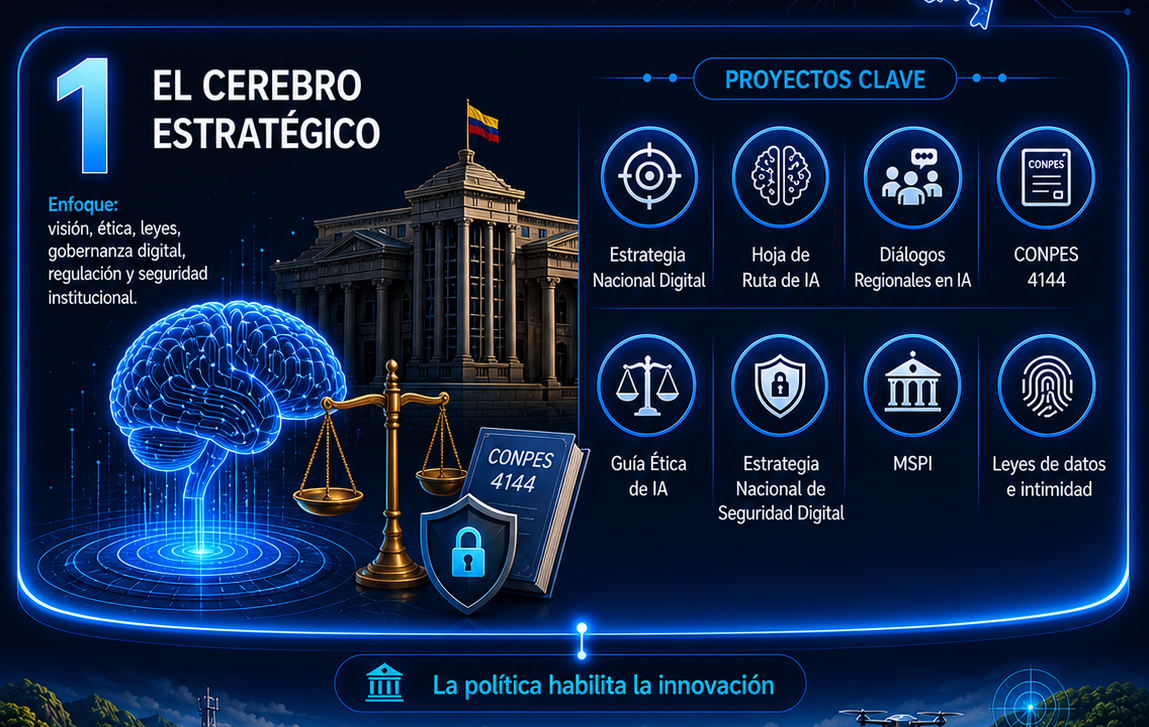
\includegraphics[width=\columnwidth]{figures/Capa1c.png}
    \caption{Capa 1 del sistema}
    \label{fig:capa1}
\end{figure}


\section{Infraestructura, Datos e Interdependencia}

La soberanía digital se construye, en primer lugar, sobre infraestructura. Sin conectividad efectiva, cualquier estrategia de transformación digital resulta limitada. La subasta 5G constituye un punto de inflexión por su dimensión tecnológica y por su orientación redistributiva, mientras el inicio oficial del despliegue en febrero de 2024 habilitó a los operadores ganadores para activar redes de quinta generación \parencite{mintic_despliegue_5g_2024}. La rendición de cuentas de MinTIC reportó para 2024 cerca de tres millones de nuevas personas conectadas, 1.353 estaciones base 5G, 909 Juntas de Internet, 78.060 computadores entregados y 2.375 antenas instaladas \parencite{mintic_rendicion_cuentas_2024}.

No obstante, en la economía digital contemporánea la infraestructura de conectividad es solo una dimensión del poder. El control, almacenamiento y procesamiento de datos emergen como elementos centrales. En el frente estatal, el Gobierno ha anunciado proyectos de centros de datos asociados a una nube soberana y al desarrollo de capacidades para inteligencia artificial. Las fuentes disponibles mencionan infraestructura en el Caribe colombiano, participación de actores internacionales como G42 y soporte de conectividad atribuido a InterNexa, aunque no todos los detalles de presupuesto, capacidad y gobernanza han sido publicados de forma completa \parencite{dcd_colombia_emiratos_datacenters_2025,presidencia_data_center_santa_marta_2025,minciencias_revolucion_cientifica_2025}.

La Convocatoria 46 del Sistema General de Regalías, denominada ``Colombia Inteligente: Infraestructura para el desarrollo de la IA'', constituye otro esfuerzo importante. La convocatoria abrió en octubre de 2025, cerró en noviembre del mismo año, contempló 630.000 millones de pesos y exigió condiciones técnicas tipo centro de datos Tier III, eficiencia energética, escalabilidad, ciberseguridad y continuidad operativa \parencite{minciencias_colombia_inteligente_2025}. El proceso también generó debate público sobre gobernanza y transparencia, lo que muestra que la soberanía digital requiere capacidades técnicas y reglas claras de contratación \parencite{lorduy_colombia_inteligente_2026}.

En paralelo, la expansión privada es significativa. ODATA anunció los campus BG02 y BG03 en Cundinamarca, con capacidad combinada de 144 MW e inversión estimada de 1.300 millones de dólares \parencite{dcd_odata_data_centers_2024,lorduy_odata_hub_tecnologia_2024}. También se identifican proyectos como Data Horizon Americas en la Zona Franca de Occidente, infraestructura de HostDime en Tocancipá, expansión de IFX Networks en Bogotá y soluciones de soberanía de datos impulsadas por Ilkari y Huawei \parencite{say_global_2026,hostdime_colombia_data_center_2026,smith_internexa_hostdime_2025,itsitio_ifx_data_center_2023,ilkari_huawei_data_center_2024}.

En términos de política pública, estas dinámicas se articulan con la Estrategia Nacional Digital 2023--2026, que incluye conectividad, datos, seguridad, talento digital, inteligencia artificial, transformación pública y economía digital \parencite{mintic_estrategia_nacional_digital_2023}. A la vez, el CONPES 4144 define una hoja de ruta de inteligencia artificial con más de 100 acciones hacia 2030 e inversión estimada de 479.000 millones de pesos \parencite{vanegas_conpes_4144_2025}. El resultado no es aislamiento tecnológico, sino una inserción estratégica donde el Estado intenta mejorar su capacidad de decisión dentro de redes globales.

Desde el enfoque de interdependencia compleja, este conjunto de iniciativas evidencia que el sistema digital colombiano no se construye en aislamiento, sino dentro de redes densas de actores públicos y privados, nacionales e internacionales. La participación de empresas como ODATA, Huawei o G42, junto con la acción estatal, muestra que la infraestructura digital y los datos dependen de múltiples niveles de interacción, donde el poder no está concentrado exclusivamente en el Estado, sino distribuido según el acceso a recursos tecnológicos, capacidades de inversión y control de información.

Sin embargo, desde la perspectiva de dependencia y desarrollo, esta inserción en redes globales también revela límites estructurales. Si bien Colombia avanza en infraestructura y capacidades en inteligencia artificial y almacenamiento de datos, buena parte de estos procesos continúa articulada a capital, tecnología y conocimiento externo. Por ello, la soberanía digital colombiana no expresa autonomía plena, sino una autonomía relativa todavía en construcción. Iniciativas como la nube soberana, los centros de datos y las políticas de inteligencia artificial apuntan a fortalecer capacidades técnicas, pero también a aumentar el control sobre recursos estratégicos como los datos, que en la economía digital contemporánea constituyen una fuente central de poder.

\section{Gobernanza, Talento y Servicios Digitales}

La soberanía digital no se limita a infraestructura: también implica capacidad para establecer reglas. La Guía Ética para la implementación, desarrollo y uso de sistemas de inteligencia artificial en entidades públicas y la actualización del Modelo de Seguridad y Privacidad de la Información refuerzan la dimensión normativa de esta transformación \parencite{dnp_guia_etica_ia_2025,mintic_guia_etica_ia_2026,mintic_mspi_resolucion_02277_2025}. La Estrategia Nacional de Seguridad Digital 2025--2027, presentada por MinTIC y ColCERT, responde a un contexto de amenazas digitales crecientes y prioriza resiliencia institucional \parencite{mintic_seguridad_digital_2025}.

La sostenibilidad de la estrategia depende además del capital humano. Talento Tech fue lanzado con una meta de formar 180.000 personas mediante bootcamps de 120 a 159 horas \parencite{mintic_talento_tech_lanzamiento_2023}. La primera adjudicación regional permitió iniciar ejecución para 18.374 personas y reportó más de 74.000 inscritos \parencite{mintic_talento_tech_regiones_2023}.

Así mismo, el Programa Orquídeas ha financiado proyectos de investigación, fortalecido vocaciones científicas y promovido la participación de mujeres en áreas estratégicas como inteligencia artificial y bioeconomía, articulando equidad y desarrollo territorial. Entre 2023 y 2025 vinculó 745 mujeres, movilizó una inversión aproximada de 84.513 millones de pesos e impactó 30 departamentos y 130 municipios \parencite{minciencias_orquideas_2025}. En esta misma línea, el Museo Virtual del Centro Nacional de Memoria Histórica constituye una plataforma digital inmersiva que permite recorrer cerca de 300 lugares de memoria construidos por víctimas del conflicto armado. La plataforma integra testimonios y archivos mediante tecnologías como IPFS, blockchain e inteligencia artificial, y fue seleccionada dentro del Top 10 mundial en la categoría de Innovación Digital de una convocatoria global de la Organización de las Naciones Unidas para el Desarrollo Industrial en 2025 \parencite{unido_innovacion_digital_2025}.

Este componente es clave porque la soberanía digital no solo implica acceso a infraestructura, sino capacidad social para usarla, producir conocimiento y participar en la economía digital.

En servicios digitales, la Agencia Nacional Digital reportó avances en Carpeta Ciudadana y REDAM, con millones de certificados expedidos y mejoras de operación \parencite{and_informe_gestion_2024}. La DIAN, por su parte, reportó uso masivo de información exógena, validación de identidad, servicios sugeridos y datos del Sistema de Facturación Electrónica \parencite{dian_informe_gestion_2025,dian_cifras_sfe_2026}. Estas herramientas fortalecen la interacción entre Estado y ciudadanía, y también amplían la capacidad estatal de gestión de información y recaudo.

Desde el enfoque de interdependencia compleja, estos avances muestran que la soberanía digital no depende únicamente del control de infraestructura, sino de la capacidad del Estado para establecer reglas, coordinar actores y gestionar riesgos en entornos altamente interconectados. La construcción de marcos éticos para la inteligencia artificial, estrategias de seguridad digital y modelos de protección de la información refleja que el poder también se ejerce a través de normas y estándares que organizan el funcionamiento del ecosistema digital.

Al mismo tiempo, desde la perspectiva de dependencia y desarrollo, el fortalecimiento del talento digital y de las capacidades institucionales puede interpretarse como una estrategia para reducir brechas estructurales. La formación de capital humano, a través de programas como Talento Tech o iniciativas de inclusión como Orquídeas, amplía las oportunidades de participación en la economía digital y contribuye a disminuir la dependencia de conocimiento y capacidades externas, uno de los rasgos históricos de las economías latinoamericanas.

En este sentido, la soberanía digital articula tres dimensiones: regulación, capacidades humanas y provisión de servicios. El Estado establece marcos normativos para ordenar el uso de tecnologías emergentes, invierte en formación de talento para garantizar apropiación social y fortalece servicios digitales para mejorar la relación entre ciudadanía y Estado. Esta combinación incrementa la eficiencia administrativa, amplía la presencia estatal en el entorno digital y consolida los datos como recurso estratégico para la gestión pública.

% \section{Aportes de MinCiencias a Tecnologías Digitales, Inteligencia Artificial y Tecnologías Cuánticas}

La contribución de MinCiencias a la soberanía digital durante el periodo analizado se concentra en tres frentes: la construcción de política pública para inteligencia artificial, la financiación de investigación aplicada en tecnologías digitales y la formación de capacidades científicas en territorios con brechas históricas. La Hoja de Ruta para el desarrollo y aplicación de la inteligencia artificial, presentada en febrero de 2024, organizó cinco entornos de trabajo: ética y gobernanza; educación, investigación e innovación; industrias innovadoras y emergentes; datos y organizaciones; y privacidad, ciberseguridad y defensa \parencite{minciencias_hoja_ruta_ia_pdf_2024,minciencias_informe_gestion_2024_pdf}. Este instrumento sirvió como insumo para la formulación del CONPES 4144, que fija una política nacional de IA con 106 acciones hasta 2030 y una inversión aproximada de 479.273 millones de pesos \parencite{conpes_4144_ia_pdf_2025}.

La dimensión participativa de esta agenda se evidencia en los Diálogos Regionales en Inteligencia Artificial. Entre abril y mayo de 2024, MinCiencias realizó encuentros en Tumaco, Bucaramanga, Villavicencio, Medellín, Yopal, Barranquilla, San Andrés, Ibagué, Zipaquirá, Duitama, Montería, Pereira y Cali, con 3.173 personas registradas. El objetivo fue diagnosticar conocimiento, apropiación, barreras y posibles soluciones territoriales basadas en IA, involucrando academia, comunidad científica, sector productivo, entidades públicas y sociedad civil \parencite{minciencias_dialogos_ia_pdf_2024}.

En financiación de proyectos, el programa ColombIA Inteligente constituye el núcleo más directamente asociado con IA, tecnologías aeroespaciales y tecnologías cuánticas. La Convocatoria 950 de 2024 financió cinco proyectos de I+D+i para soluciones mediante inteligencia artificial y ciencias del espacio, con 6.627 millones de pesos de MinCiencias y 1.889 millones de contrapartidas. Además, vinculó capacidades de talento mediante 40 jóvenes investigadores, 7 estudiantes de maestría y 3 estancias posdoctorales \parencite{minciencias_rendicion_2024_2025_pdf}. La Convocatoria 966 de 2025 amplió el alcance hacia ciencias y tecnologías cuánticas e inteligencia artificial; abrió el 25 de abril de 2025, cerró el 18 de junio de 2025 y tenía previsto publicar resultados definitivos en septiembre de 2025 \parencite{minciencias_rendicion_2024_2025_pdf}.

La agenda también incluye apropiación tecnológica temprana. Colombia Robótica desarrolló campamentos STEAM en 2024 con 1.200 niños, niñas y adolescentes y 80 docentes beneficiados, en Antioquia, Cundinamarca y Tumaco, con actividades en programación, robótica, diseño, realidad virtual e inteligencia artificial. En 2025, el programa entregó y adecuó 15 laboratorios STEAM en instituciones educativas de Tumaco, con equipamiento tecnológico, mobiliario especializado, kits de robótica y material didáctico \parencite{minciencias_rendicion_2024_2025_pdf}. Adicionalmente, en la respuesta a la emergencia del Catatumbo entre el 26 de enero y el 7 de febrero de 2025, MinCiencias reportó talleres de robótica, programación, electrónica maker, astronomía y cartografía participativa, con 430 niños, niñas, adolescentes y jóvenes beneficiados, 500 kits entregados y 26 talleres realizados \parencite{minciencias_rendicion_2024_2025_pdf}.

Finalmente, Orquídeas y la convocatoria de Investigación Fundamental amplían la base de capacidades científicas que sostiene la transformación digital. Orquídeas financió 107 proyectos en su versión 2023 por 20.611 millones de pesos y proyectó 119 proyectos en 2024 por 28.702 millones, vinculando doctoras y jóvenes investigadoras a proyectos de I+D+i con enfoque territorial y de género \parencite{minciencias_informe_gestion_2024_pdf}. La Convocatoria 937 de Investigación Fundamental incluyó proyectos con aprendizaje de máquina e inteligencia artificial, como investigación sobre aleaciones con imágenes multiescala y aprendizaje de máquina, y avances terapéuticos en péptidos antimicrobianos con IA \parencite{minciencias_informe_gestion_2024_pdf}.



\section{Línea de Tiempo Integrada}

\begin{itemize}
    \item \textbf{26 de septiembre de 2022:} anuncio del campus Data Horizon Americas en la Zona Franca de Occidente, con proyección cercana a 55 MW \parencite{say_global_2026}.
    \item \textbf{30 de junio de 2023:} Decreto 1079, que regula el Internet Comunitario Fijo \parencite{funcionpublica_decreto_1079_2023}.
    \item \textbf{14 de septiembre de 2023:} lanzamiento de Talento Tech \parencite{mintic_talento_tech_lanzamiento_2023}.
    \item \textbf{20 de diciembre de 2023:} subasta 5G con obligaciones de hacer orientadas a conectividad rural \parencite{mintic_5g_realidad_2023}.
    \item \textbf{23 de febrero de 2024:} resoluciones que habilitan el despliegue oficial de redes 5G \parencite{mintic_despliegue_5g_2024}.
    \item \textbf{7 de octubre de 2024:} MinTIC informa avances en construcción de data center para inteligencia artificial \parencite{mintic_data_center_ia_2024}.
    \item \textbf{23 de octubre de 2024:} ODATA anuncia los campus BG02 y BG03 en Cundinamarca \parencite{dcd_odata_data_centers_2024}.
    \item \textbf{9 de diciembre de 2024:} rendición de cuentas de MinTIC con avances en conectividad, equipos y 5G \parencite{mintic_rendicion_cuentas_2024}.
    \item \textbf{20 de diciembre de 2024:} lanzamiento del Centro de Monitoreo e Inspección de Servicios de Comunicaciones \parencite{mintic_cmic_telecomunicaciones_2024}.
    \item \textbf{Febrero de 2025:} reporte y comunicaciones sobre centros de datos en el Caribe colombiano y cooperación con G42 \parencite{dcd_colombia_emiratos_datacenters_2025,minciencias_revolucion_cientifica_2025}.
    \item \textbf{14 de febrero de 2025:} aprobación del CONPES 4144 de inteligencia artificial \parencite{vanegas_conpes_4144_2025}.
    \item \textbf{28 de marzo de 2025:} Resolución CRC 7712 sobre regulación diferencial para Internet Comunitario Fijo \parencite{crc_resolucion_7712_2025}.
    \item \textbf{3 de junio de 2025:} Resolución 02277 actualiza el MSPI y lo alinea con ISO/IEC 27001:2022 \parencite{mintic_mspi_resolucion_02277_2025}.
    \item \textbf{24 de junio de 2025:} presentación de la Estrategia Nacional de Seguridad Digital 2025--2027 \parencite{mintic_seguridad_digital_2025}.
    \item \textbf{30 de septiembre de 2025:} HostDime reporta la integración de un Mega PoP de InterNexa en su data center Nebula \parencite{smith_internexa_hostdime_2025}.
    \item \textbf{14 de octubre de 2025:} apertura de la Convocatoria 46 del SGR para infraestructura de IA \parencite{minciencias_colombia_inteligente_2025}.
\end{itemize}

La integración de estos hitos muestra una secuencia acumulativa en la que regulación, infraestructura, talento y gobernanza avanzan de forma paralela. En términos de Keohane y Nye, Colombia no se aísla, sino que fortalece su capacidad de decisión dentro de redes globales mediante inversión, regulación y cooperación \parencite{keohane_nye_power_2011}.

Desde el enfoque de interdependencia compleja, la línea de tiempo refleja una estrategia de inserción activa en redes globales, más que un intento de aislamiento tecnológico. La participación de actores internacionales en proyectos de infraestructura, junto con el desarrollo de marcos regulatorios y capacidades internas, indica que Colombia busca mejorar su posición relativa dentro de estas redes, aumentando su capacidad de negociación, regulación y toma de decisiones.

Desde la perspectiva de dependencia y desarrollo, la secuencia también puede interpretarse como un esfuerzo por reducir vulnerabilidades estructurales. La inversión en talento digital, la regulación del internet comunitario y el impulso a infraestructura de datos muestran intentos por fortalecer capacidades internas históricamente limitadas en la región. No obstante, el hecho de que varios avances se articulen con capital y tecnología externa evidencia que la autonomía alcanzada es relativa y se construye dentro de condiciones de dependencia persistentes.

\section{Riesgos y Consideraciones}

A pesar de los avances, la consolidación de la estrategia digital ocurre en un contexto de desafíos estructurales. En el plano económico, proyectos de gran escala liderados por actores como ODATA pueden fortalecer a Colombia como hub digital regional, pero la evidencia pública sobre empleo, encadenamientos productivos, consumo energético, agua y huella ambiental todavía es heterogénea. La discusión regional sobre centros de datos muestra que las promesas de inversión no siempre se acompañan de datos comparables sobre impactos sociales y ambientales \parencite{aosfatos_data_centers_latam_2025}.

El componente energético es estratégico. Proyectos como BioNube, con requerimientos estimados de decenas de MW, y los desarrollos privados con conexión directa a redes de transmisión evidencian que la expansión de infraestructura digital depende de energía confiable, sostenible y competitiva. Los cuellos de botella no se limitan a suelo o conectividad: incluyen capacidad energética, gestión hídrica y eficiencia de refrigeración.

En soberanía y gobernanza de datos, la nube soberana y los estándares técnicos de infraestructura apuntan a fortalecer control nacional, pero su implementación plantea retos: dependencia de proveedores internacionales, transferencia efectiva de conocimiento, reglas de custodia, acceso, auditoría y mecanismos de supervisión. La confianza pública depende de marcos de gobernanza claros, especialmente cuando participan actores extranjeros o esquemas público-privados.

En conectividad, los resultados documentados reflejan avances en cobertura, estaciones base 5G, redes comunitarias y entrega de dispositivos. Sin embargo, persisten brechas de acceso que limitan la captura plena de beneficios. Además, situaciones administrativas asociadas a operadores específicos de la subasta 5G muestran la necesidad de mecanismos ágiles para gestionar contingencias y asegurar cumplimiento \parencite{mintic_telecall_espectro_5g_2025,lorduy_telecall_conciliacion_2026}.

En gobierno digital y servicios, el desafío consiste en complementar indicadores de producto con mediciones de impacto. La propia planeación sectorial reconoce la importancia de medir resultados más allá de entregables, incluyendo adopción efectiva, calidad, satisfacción, empleabilidad y valor público \parencite{mintic_indicadores_impacto_2026}. En inteligencia artificial, el reto es pasar de principios y guías a reportes verificables de riesgo, datos utilizados, explicabilidad, sesgos, mecanismos de queja y presupuestos ejecutados.

% \section{Recomendaciones}

% Primero, se recomienda crear un tablero público unificado de metas digitales del cuatrienio, alineado con la Estrategia Nacional Digital 2023--2026. Cada iniciativa debería incluir línea base, metas anuales, avances verificables, responsables, presupuesto y fuente documental.

% Segundo, conviene normalizar indicadores de impacto. En conectividad y formación, no basta medir cobertura o cupos: se requiere evaluar adopción efectiva, calidad del servicio, resultados educativos, empleabilidad, asequibilidad y satisfacción de usuarios.

% Tercero, para 5G y obligaciones de hacer, se debería publicar información desagregada por institución educativa, municipio y operador: estado de implementación, cronograma, contingencias y evidencia de operación. En conectividad comunitaria, el Decreto 1079 y la Resolución 7712 deberían complementarse con evaluaciones periódicas de sostenibilidad, costos por hogar, calidad, gobernanza local y barreras regulatorias \parencite{funcionpublica_decreto_1079_2023,crc_resolucion_7712_2025}.

% Cuarto, en inteligencia artificial pública, toda implementación debería reportar cumplimiento de la Guía Ética, incluyendo evaluación de riesgos, características de los datos, explicabilidad, desempeño, sesgos, mecanismos de rendición de cuentas y presupuesto ejecutado \parencite{dnp_guia_etica_ia_2025,mintic_guia_etica_ia_2026}.

% Quinto, dada la relevancia de la infraestructura de datos, se requieren fichas técnicas estandarizadas para proyectos de centros de datos con participación estatal o incentivos públicos. Estas fichas deberían incluir capacidad, fases de desarrollo, certificaciones, eficiencia energética, suministro eléctrico, uso de agua, empleo, inversión ejecutada y reglas de gobernanza de datos.



%%%%%%%%%%%% GRAFICOS CAPAS

% capa 1: 

% Estrategia Nacional Digital
% Hoja de ruta de la IA
% CONPES 4144
% Guía ética de la IA
% Estrategia de Seguridad Nacional
% MSPI
% Ley de Datos e Intimidad
% Comunidades de Conectividad
% Internet comunitario


% capa 2:
% Colombia inteligente: Tecnologías Cuánticas
% Colombia inteligente: Inteligencia Artificial
% Colombia Inteligente: Ciencias espaciales
% Software propio (Ejército)
% Ciencia Marítima (Armada)
% Tecnología antidrones
% Dialogos regionales IA y Cuántica


% Capa 3:
% Inlcuir
% 	AvanzaTec
% 	Plan Pescador(Ejército)
% 	Ciberpaz
% 	Ciencia para la paz (Catatumbo)
	
% capa 4.
% quitar: drones, redes de defensa
% Conectividad PDET Frontera
% conectiVIDAd: Chocó Nariño Guajira
% Internet Rural
% quitar DIAN digital







\section{Conclusiones}
La soberanía digital se ha convertido en una dimensión indispensable de la soberanía estatal contemporánea. En un contexto en el que el ciberespacio concentra buena parte de la interacción social, el acceso a servicios, la circulación de información, la participación política y el ejercicio de derechos fundamentales, los Estados ya no pueden limitar su acción al territorio físico. Deben proyectar su capacidad de regulación, protección y garantía de derechos hacia el entorno digital. En el caso colombiano, esta tarea adquiere un sentido particular: en un Estado social de derecho, donde la soberanía emana del pueblo, la soberanía digital debe entenderse como una condición para ampliar la ciudadanía, reducir desigualdades y garantizar que las personas puedan ejercer sus derechos también en el plano virtual.

Desde esta perspectiva, la soberanía digital no se reduce a la ciberseguridad, al control de datos o al despliegue de infraestructura tecnológica. Estos elementos son necesarios, pero insuficientes. La experiencia analizada muestra que una política digital con sentido democrático debe articular infraestructura, regulación, capacidades institucionales, formación, acceso territorial y participación comunitaria. Por ello, el periodo 2022–2026 puede interpretarse como un momento de inflexión en el que la transformación digital comienza a ser entendida no solo como modernización administrativa o competitividad económica, sino como una herramienta de equidad, inclusión y fortalecimiento del Estado social.

Las acciones desarrolladas durante el gobierno de Gustavo Petro evidencian una apuesta por orientar la política digital hacia poblaciones y territorios históricamente excluidos. El fortalecimiento de sistemas de información estratégicos, la inversión en centros de datos y capacidades asociadas a inteligencia artificial, la expansión de conectividad rural, las obligaciones sociales vinculadas al despliegue 5G, los programas de formación digital y las iniciativas de apropiación tecnológica muestran una visión más amplia de la soberanía digital. En ella, el Estado no solo busca mejorar su capacidad técnica, sino también extender su presencia, proteger derechos y habilitar nuevas formas de participación social.

El análisis por capas permite observar con mayor claridad esta arquitectura. La primera capa muestra el avance normativo e institucional necesario para ordenar el ecosistema digital, desde estrategias nacionales hasta lineamientos de inteligencia artificial, seguridad digital y gobernanza de datos. La segunda capa evidencia el impulso a la investigación, la innovación y las capacidades científicas en áreas como inteligencia artificial, tecnologías cuánticas, robótica y ciencia de datos. La tercera capa expresa la dimensión social de la política digital, al incorporar programas dirigidos a mujeres, niñas, niños, jóvenes, comunidades rurales, territorios de frontera y zonas afectadas por el conflicto. Finalmente, la cuarta capa muestra la importancia de una infraestructura incluyente, capaz de llevar conectividad, dispositivos, centros de datos, redes comunitarias y servicios digitales a territorios donde la brecha tecnológica ha coincidido históricamente con otras formas de exclusión.

Uno de los aportes más relevantes del periodo es la incorporación de las comunidades como actores activos de la conectividad. La regulación diferencial para el Internet Comunitario Fijo y el reconocimiento de organizaciones sociales, juntas de acción comunal y comunidades organizadas como posibles prestadoras de servicios digitales abren una vía distinta para resolver los problemas de última milla. Esta orientación desplaza parcialmente la política digital desde una lógica exclusivamente centralizada o de mercado hacia una lógica de apropiación territorial, sostenibilidad comunitaria y corresponsabilidad social. En ese sentido, la soberanía digital también se construye desde abajo, mediante capacidades locales y formas comunitarias de gestión tecnológica.

Con todo lo anterior, y pese a las ventajas que ofrecen los avances identificados, persisten desafíos estratégicos para la consolidación de una soberanía digital más profunda. El primero es superar el rezago tecnológico mediante el fortalecimiento, público y privado, de capacidades nacionales en sectores digitales de alto valor, especialmente en la producción, diseño, mantenimiento y apropiación de tecnologías asociadas a semiconductores, chips y componentes críticos. Sin estas capacidades, la autonomía relativa alcanzada seguirá dependiendo en buena medida de proveedores, capitales y cadenas globales externas.

Un segundo desafío es la masificación del software libre, aspecto todavía poco visible en esta primera etapa de transformación digital. Su ausencia parcial puede explicarse por las barreras culturales, institucionales y técnicas que implica migrar hacia modelos abiertos. Sin embargo, una estrategia de soberanía digital debería avanzar en dos direcciones complementarias: ampliar el uso de software libre en entidades públicas, procesos educativos y proyectos comunitarios, y promover la producción nacional de soluciones abiertas, así como la participación de talento colombiano en comunidades y proyectos internacionales de software libre.

El tercer desafío se relaciona con el poder creciente de las grandes plataformas digitales y redes sociales, cuya concentración económica, algorítmica y comunicativa configura una suerte de “monarquía digital” \parencite{peirano_enemigo_nodate}. Este poder incide sobre la circulación de información, la formación de opinión pública, la privacidad, la deliberación democrática y la autonomía de los ciudadanos en el entorno digital. Por ello, una política de soberanía digital no puede limitarse a infraestructura, conectividad o servicios estatales: también debe enfrentar los riesgos derivados de la dependencia de plataformas privadas globales que median buena parte de la vida pública contemporánea.


Desde la perspectiva de las relaciones internacionales, la estrategia colombiana puede entenderse como un intento de reposicionamiento dentro del sistema global. En lugar de buscar autonomía absoluta, el país avanza hacia una forma de interdependencia regulada: fortalece su capacidad de decisión sin romper con redes globales de capital, datos y tecnología.

El caso colombiano combina inversión pública, regulación, cooperación internacional y atracción de capital privado global. La coexistencia de iniciativas de nube soberana con inversión extranjera en data centers, junto con la adopción de estándares internacionales, muestra una estrategia de inserción activa. En este marco, la soberanía no implica aislamiento, sino capacidad de influir, regular, negociar y reducir vulnerabilidades dentro de redes densamente interconectadas \parencite{keohane_nye_power_2011}.

El modelo adoptado por Colombia combina inversión pública, fortalecimiento regulatorio, cooperación internacional y atracción de capital privado global. La coexistencia de iniciativas como la nube soberana con la expansión de infraestructura impulsada por actores internacionales, así como la adopción de estándares globales, evidencia una estrategia pragmática que busca ampliar márgenes de autonomía sin romper con las dinámicas del sistema internacional. Desde la perspectiva de Cardoso y Faletto, este proceso puede interpretarse como la construcción de una autonomía relativa, en la que el Estado intenta reconfigurar su posición dentro de estructuras de dependencia históricas \parencite{cardoso_faletto_dependencia_1977}.

El periodo 2022--2026 marca un punto de inflexión en la política digital de Colombia. La transformación no se limita a la adopción tecnológica, sino a la redefinición del rol del Estado, que pasa de ser un actor principalmente regulador a uno que también promueve capacidades, coordina actores y amplía su presencia en el entorno digital. Al articular infraestructura, datos, gobernanza, talento y desarrollo social, el país comienza a consolidar una soberanía digital pragmática, orientada tanto al fortalecimiento estatal como a la reducción de brechas sociales y territoriales.

En este contexto, la soberanía digital adquiere una dimensión social: no solo se trata de controlar o regular tecnologías, sino de garantizar acceso, formar capacidades y promover la participación de sectores históricamente excluidos. De este modo, la expansión de la conectividad, el desarrollo de talento digital y la provisión de servicios públicos digitales no solo mejoran la eficiencia del Estado, sino que también fortalecen el capital humano y amplían las oportunidades de inclusión en la economía digital colombiana.


% \section{Defensa}

 Seguridad, defensa y soberanía digital en Colombia
Resultados del Ministerio de Defensa, el Ejército Nacional, la Fuerza Aeroespacial Colombiana, la Armada Nacional y la Policía Nacional en materia digital 
La soberanía digital en Colombia encuentra en el sector defensa uno de sus espacios más concretos de materialización, en la medida en que la capacidad estatal no se limita a la formulación normativa, sino que se traduce en control efectivo sobre infraestructuras, datos y dinámicas de riesgo en el ciberespacio. Desde la perspectiva de Robert Keohane y Joseph Nye, este proceso puede entenderse como un intento por gestionar la interdependencia global en términos de vulnerabilidad y capacidad de ajuste. En un entorno caracterizado por flujos constantes de información y amenazas transnacionales, el problema no es la conexión en sí misma, sino los costos a la exposición diferencial \parencite{keohane_nye_power_2011,mintic_seguridad_digital_2025}.

En este contexto, las Fuerzas Militares y la Policía han desarrollado una arquitectura de ciberdefensa basada en monitoreo, prevención y respuesta que refleja un tránsito desde esquemas reactivos hacia modelos anticipativos de gestión del riesgo. La implementación de sistemas SIEM para análisis predictivo, soluciones WAF para la protección de aplicaciones críticas, firewalls dinámicos para segmentación de tráfico y tecnologías Anti-DDoS de nueva generación respaldadas por inversiones superiores a 9.006 millones de pesos en herramientas de seguridad y más de 4.142 millones de pesos en capacidades de monitoreo y forense digital no solo amplía la capacidad técnica del Estado, sino que reduce su vulnerabilidad estructural frente a eventos externos. En términos de interdependencia compleja, estas capacidades no eliminan la exposición a amenazas globales, pero sí disminuyen los costos asociados a ellas al mejorar la capacidad de respuesta y adaptación \parencite{mindefensa_audiencia_rendicion_2025,cogfm_informe_ejecutivo_2025}.
Este proceso se profundiza con el desarrollo de tecnologías de decepción cibernética, con inversiones cercanas a 2.369 millones de pesos, orientadas a la creación de entornos simulados que permiten identificar patrones de comportamiento malicioso.  \parencite{mindefensa_audiencia_rendicion_2025}.

Sin embargo, estos avances no pueden entenderse únicamente desde la lógica de la interdependencia. Desde la perspectiva de Fernando Henrique Cardoso y Enzo Faletto, el problema central no es solo la exposición a riesgos externos, sino la posición estructural que ocupa el país en el sistema tecnológico global. En este sentido, la construcción de capacidades de ciberdefensa puede interpretarse también como un intento de reducir la dependencia tecnológica, en la medida en que fortalece el control nacional sobre infraestructuras críticas y procesos de decisión. No obstante, esta reducción es parcial: las tecnologías utilizadas, los estándares y gran parte de los ecosistemas digitales continúan anclados en redes globales dominadas por actores externos, lo que sugiere que la soberanía digital se configura como una autonomía relativa más que como independencia plena \parencite{cardoso_faletto_dependencia_1977}.

Estas capacidades técnicas se articulan con una gobernanza institucional ampliada del ciberespacio, caracterizada por la coordinación entre múltiples entidades estatales. La activación del PMU Ciber electoral, con la participación de ocho entidades, evidencia la creciente centralidad de la seguridad digital en la protección de procesos democráticos y confirma la existencia de múltiples canales de interacción uno de los rasgos centrales de la interdependencia compleja en los que actores estatales, agencias especializadas y organismos internacionales participan simultáneamente en la gestión del riesgo \parencite{mindefensa_audiencia_rendicion_2025,mintic_seguridad_digital_2025}.

De manera complementaria, el Centro Cibernético Policial ha consolidado una capacidad operativa significativa, reflejada en 17.321 bloqueos preventivos de páginas web (12.210 asociadas a abuso sexual infantil y 5.111 a juegos ilegales), la atención de 11.373 incidentes informáticos mediante el CAI Virtual, la emisión de 245 alertas preventivas en redes sociales, la identificación de 67 riesgos cibernéticos y la detección de 2.149 intentos de phishing dirigidos a entidades públicas y privadas. Estas acciones se complementan con operaciones bajo la estrategia ESCIB--C2, que han derivado en 46 capturas (31 por delitos informáticos y 15 por explotación sexual infantil). Además ha desarrollado el desarrollo del Plan Pescador, que ha permitido la incautación de dispositivos, el análisis forense digital y la judicialización de redes criminales relacionadas a la explotación infantil en entornos digitales en cooperación con agencias internacionales como Homeland Security Investigations (HSI) y el Centro Nacional para Niños Desaparecidos y Explotados (NCMEC) \parencite{policia_rendicion_logros_retos_2025,policia_plan_pescador_ninez_digital}.

Más allá de su dimensión operativa, este conjunto de acciones evidencia que la soberanía digital no se ejerce únicamente mediante infraestructura tecnológica, sino a través de la capacidad de ejercer autoridad efectiva en el ciberespacio. En términos analíticos, esto implica que el poder estatal no se define por el aislamiento de las redes globales, sino por la capacidad de intervenir en ellas, regular sus efectos y proteger a la ciudadanía en entornos digitales. Así, la soberanía digital en Colombia emerge como un proceso híbrido en el que la gestión de la interdependencia y la reducción de la dependencia se articulan para ampliar el margen de acción del Estado dentro de un sistema internacional altamente interconectado.

En paralelo, el sector defensa ha avanzado en la construcción de soberanía tecnológica mediante el desarrollo de software propio, un proceso que puede interpretarse como un intento de reducir la dependencia de proveedores externos y fortalecer el control estatal sobre información estratégica. herramientas como CAOCC PDF,  la plataforma ORIÓN para cesantías,  el sistema SIJEN para procesos disciplinarios,  y la modernización de SISPRO, con 108 millones de pesos. A estos desarrollos se suman SICOE 2.0 para analítica de datos en tiempo real,  y sistemas de gestión de casinos  \parencite{mindefensa_audiencia_rendicion_2025,cogfm_informe_ejecutivo_2025}.

Este proceso se complementa con la modernización del sistema de reclutamiento interoperable con la Registraduría Nacional, la implementación de la plataforma SGDEA para gestión documental interoperable entre fuerzas, el desarrollo de aplicaciones móviles como PadillApp en la Armada Nacional y la incorporación de chatbots institucionales en la Fuerza Aeroespacial Colombiana. En conjunto, estas iniciativas evidencian un tránsito progresivo hacia la producción interna de tecnología;  \parencite{arc_informe_rendicion_2023,fac_informe_rendicion_2023,cardoso_faletto_dependencia_1977}.

El fortalecimiento de la infraestructura tecnológica constituye otro eje central de esta estrategia y refuerza esta lógica de autonomía relativa. El sector defensa ha expandido sus redes de comunicación hasta alcanzar capacidades de 400 Gbps, y su capacidad de respaldo de datos de 40 TB a 223 TB, . Estas capacidades se acompañan de inversiones de 8.598 millones de pesos en redes integradas, 2.734 millones de pesos en redes de alta velocidad y 2.869 millones de pesos en sistemas de comunicaciones como FREQUENTIS, junto con la distribución de 1.849 computadores para fortalecer capacidades operativas y administrativas. En el ámbito naval, estos avances se complementan con la implementación de comunicaciones satelitales mediante sistemas Iridium, el despliegue de fibra óptica en zonas remotas, la modernización de sistemas de vigilancia marítima con inversiones superiores a 3.700 millones de pesos y la adopción de sistemas de videoconferencia institucional con inversiones cercanas a 1.498 millones de pesos \parencite{mindefensa_audiencia_rendicion_2025,arc_informe_rendicion_2023,cogfm_informe_ejecutivo_2025}.

Desde la perspectiva de la interdependencia compleja, estas inversiones no eliminan la exposición del Estado a redes globales, pero sí reducen su vulnerabilidad al mejorar su capacidad de ajuste frente a perturbaciones externas. En términos de Robert Keohane y Joseph Nye, la infraestructura digital no rompe la interdependencia, sino que la hace más manejable, al disminuir los costos asociados a fallas, ataques o interrupciones en los flujos tecnológicos. Así, la construcción de una base material robusta no implica aislamiento, sino resiliencia dentro de sistemas interconectados \parencite{keohane_nye_power_2011}.

El componente de innovación tecnológica refuerza esta transformación al evidenciar un tránsito hacia la producción de capacidades estratégicas propias. La operación del satélite FACSAT-2 permitió la captura de 725 imágenes, de las cuales 659 fueron procesadas para misiones de inteligencia y gestión del riesgo, mientras que proyectos como el Ala Zagi desarrollaron aeronaves autónomas de bajo costo para vigilancia. Paralelamente, el sector defensa consolidó una flota de 966 drones para inteligencia, reconocimiento y operaciones, desarrolló sistemas antidrones como NESHER V4 con patentes propias, ensambló sistemas de detección y neutralización e incorporó tecnologías GNSS RTK para la calibración de navegación aérea. Estas capacidades se articulan con la adopción de inteligencia artificial en procesos institucionales, el uso de analítica de datos en tiempo real mediante herramientas como Power BI, la implementación de simulaciones de realidad virtual para entrenamiento y el desarrollo de investigaciones en IA aplicada a educación y gestión institucional \parencite{fac_informe_rendicion_2023,mindefensa_audiencia_rendicion_2025,mindefensa_100_logros_2026}.

Más que un proceso de adopción tecnológica, este conjunto de iniciativas puede interpretarse como un intento de reposicionamiento del Estado dentro de la economía política de la tecnología. En términos de dependencia, implica avanzar aunque de manera parcial hacia la producción de conocimiento y capacidades propias; en términos de interdependencia, supone ampliar la capacidad del Estado para operar, negociar y ejercer control dentro de redes globales. En este sentido, la innovación tecnológica en el sector defensa no solo incrementa la eficiencia operativa, sino que redefine el lugar del Estado colombiano en el sistema internacional, al transformar su rol de usuario de tecnología en un actor con capacidades crecientes de producción y adaptación estratégica.
A estos avances se suma un fortalecimiento estructural de las capacidades estratégicas del Estado que amplía significativamente el alcance de la soberanía digital en Colombia. La Estrategia Nacional de Seguridad Digital 2025--2027 evidencia la magnitud del desafío al señalar que el país concentró aproximadamente el 17\% de los intentos de ciberataque en América Latina cerca de 36.000 millones de eventos en 2024, lo que ha llevado a la formulación de una respuesta institucional orientada a la creación de una entidad nacional especializada, la implementación de un Observatorio de Seguridad Digital y la adopción obligatoria de arquitecturas Confianza Cero (Zero Trust) en sistemas gubernamentales, junto con el fortalecimiento de los CSIRT bajo el modelo internacional SIM3. Desde la perspectiva de la interdependencia compleja, este conjunto de medidas refleja un intento por reducir la vulnerabilidad del Estado frente a flujos y amenazas transnacionales, no mediante el aislamiento, sino a través del fortalecimiento de su capacidad de anticipación, monitoreo y respuesta en redes altamente interconectadas. En este sentido, la estrategia no busca eliminar la interdependencia, sino hacerla más manejable y menos costosa \parencite{mintic_seguridad_digital_2025,keohane_nye_power_2011}.

En el plano operativo, el fortalecimiento de capacidades tecnológicas ha adquirido una dimensión más robusta mediante inversiones significativas en sistemas de defensa avanzada. Se destacan los 30.000 millones de pesos gestionados para el desarrollo de tecnologías anti-drones y la priorización de 126.200 millones de pesos en capacidades defensivas frente a amenazas aéreas no tripuladas, junto con la consolidación de una flota de 966 drones, incluyendo 66 modelos de alta capacidad que incrementaron el poder de fuego institucional en un 147\% \parencite{mindefensa_audiencia_rendicion_2025,mindefensa_100_logros_2026}. 
Paralelamente, el desarrollo del sistema NESHER V4 permitió la generación de capacidades propias de detección e inhibición, con 34 sistemas ensamblados y 35 detectores desplegados en zonas estratégicas, además de la neutralización efectiva de múltiples amenazas en campo. Estos avances reflejan una transición hacia un modelo de defensa tecnológica que integra capacidades digitales, físicas y operacionales, y que, desde el enfoque de la dependencia, puede interpretarse como un intento por reducir la subordinación tecnológica al desarrollar soluciones propias en ámbitos tradicionalmente dominados por proveedores externos. No obstante, esta reducción es parcial, en tanto dichas capacidades continúan insertas en cadenas globales de producción tecnológica \parencite{mindefensa_audiencia_rendicion_2025,cardoso_faletto_dependencia_1977}.

De manera complementaria, el Estado ha fortalecido su capacidad de gestión territorial y toma de decisiones mediante el uso de sistemas de información avanzados. Plataformas como el Sistema Integral de Derechos Humanos (SIDEH), que permitió el seguimiento de 1.399 activaciones de rutas de protección, el Sistema de Información de Gestión Territorial (SEGET), orientado a la priorización de inversiones, y el SIIPO para el seguimiento de compromisos del posconflicto, evidencian la incorporación de herramientas digitales en la gestión estatal y la articulación entre seguridad, desarrollo territorial y política pública. Desde la lógica de la interdependencia compleja, estos sistemas amplían la capacidad del Estado para procesar información y coordinar acciones en múltiples niveles, reduciendo la sensibilidad frente a perturbaciones externas al mejorar la capacidad de respuesta interna \parencite{mindefensa_siipo_implementacion_2025,mindefensa_audiencia_rendicion_2025}.

En el ámbito de ciencia, tecnología e innovación, la adopción de la política sectorial de CTeI mediante la Resolución 2443 de 2024 marca un punto de inflexión al establecer un enfoque orientado por misiones para cerrar brechas tecnológicas en la Fuerza Pública. Este proceso se refleja en la gestión de 94 procesos de propiedad intelectual y la obtención de 47 registros, así como en la implementación de esquemas de transferencia tecnológica que incluyen capacidades de mantenimiento de aeronaves, modernización de sistemas de comunicaciones y desarrollo de entrenamiento táctico avanzado. A ello se suma la exploración de tecnologías emergentes como la computación cuántica y la criptografía post-cuántica, lo que evidencia una estrategia orientada no solo a la adopción, sino a la producción de conocimiento tecnológico de frontera. En términos de dependencia, este giro resulta particularmente significativo, en tanto sugiere un desplazamiento aunque aún incipiente hacia la construcción de capacidades endógenas de innovación, elemento clave para modificar la posición estructural del país en la economía política global de la tecnología \parencite{mindefensa_audiencia_rendicion_2025,cogfm_informe_ejecutivo_2025}.

En conjunto, estos desarrollos muestran que la soberanía digital en Colombia se está configurando a través de una doble dinámica: por un lado, la gestión de la interdependencia mediante el fortalecimiento de capacidades de resiliencia frente a amenazas globales; por otro, la reducción parcial y progresiva de la dependencia mediante la construcción de capacidades tecnológicas propias. En este equilibrio, la soberanía no se expresa como independencia absoluta, sino como una forma de autonomía relativa que amplía el margen de acción del Estado dentro de estructuras globales interdependientes.

Finalmente, el fortalecimiento de capacidades en el dominio marítimo y científico amplía el alcance de la soberanía digital más allá del ciberespacio, evidenciando su carácter multidimensional. La incorporación del buque de investigación ARC Simón Bolívar, el desarrollo de sistemas de simulación inmersiva para entrenamiento, la implementación de sistemas de gestión de combate de fabricación nacional y el uso de tecnologías robóticas para investigación marina reflejan una integración progresiva entre defensa, ciencia y tecnología. Estas capacidades se complementan con el desarrollo de modelos predictivos para operaciones de búsqueda y rescate y el uso de herramientas digitales para el monitoreo ambiental y marítimo, configurando una forma de soberanía que no se limita al control de datos, sino que se extiende a la capacidad de producir, procesar y aplicar conocimiento en múltiples dominios estratégicos \parencite{arc_informe_rendicion_2023,mindefensa_audiencia_rendicion_2025}.

Desde la perspectiva de la interdependencia compleja, este tipo de desarrollos amplía la capacidad del Estado para operar dentro de redes globales altamente interconectadas, al reducir su vulnerabilidad frente a contingencias externas mediante el fortalecimiento de sus capacidades de respuesta y adaptación. Sin embargo, lejos de implicar un proceso de desconexión, estas capacidades confirman que la soberanía digital se construye en interacción con dichas redes, en un entorno donde la gestión del riesgo depende tanto de la articulación internacional como de la fortaleza interna \parencite{keohane_nye_power_2011}.

La transformación digital también se refleja en la relación entre el Estado y la ciudadanía, evidenciando que la soberanía digital no es exclusivamente una cuestión de seguridad, sino también de gobernanza. La digitalización permitió que el 98,5\% de las peticiones en la Fuerza Aeroespacial fueran gestionadas por canales virtuales, mientras que el portal institucional registró más de 575.000 visitas y las plataformas educativas alcanzaron capacidades superiores a 300.000 usuarios. A ello se suma la implementación de SALUD.SIS, con inversiones cercanas a 9.000 millones de pesos, que ha modernizado la prestación de servicios mediante telemedicina y telemonitoreo, así como la integración de bibliotecas digitales que conectan más de 60 unidades institucionales. En términos de transparencia, el sector alcanzó calificaciones de 93 sobre 100 en índices de acceso a la información, fortaleciendo mecanismos de participación digital y rendición de cuentas. Este conjunto de avances sugiere que la soberanía digital también se expresa en la capacidad del Estado para organizar, distribuir y garantizar el acceso a bienes públicos digitales \parencite{fac_informe_rendicion_2023,mindefensa_audiencia_rendicion_2025}.

En conjunto, estos desarrollos evidencian que la soberanía digital en Colombia no puede entenderse como independencia tecnológica absoluta, sino como la construcción de capacidades estatales orientadas a gestionar la interdependencia global y a reducir, de manera parcial, la dependencia estructural. Desde la perspectiva de Robert Keohane y Joseph Nye, estas capacidades disminuyen la vulnerabilidad del Estado frente a amenazas externas al mejorar su capacidad de ajuste, sin eliminar su inserción en redes globales. Desde el enfoque de Fernando Henrique Cardoso y Enzo Faletto, el fortalecimiento de software propio, infraestructura y capacidades tecnológicas representa un intento por desplazar, aunque de forma incompleta, los centros de decisión hacia el ámbito nacional, reconfigurando las relaciones de subordinación tecnológica \parencite{keohane_nye_power_2011,cardoso_faletto_dependencia_1977}.
En este equilibrio, la soberanía digital emerge como una forma de autonomía relativa, en la que el Estado amplía su capacidad de decisión, negociación y control dentro de estructuras interdependientes. Más que un proyecto de autosuficiencia, se trata de una estrategia de inserción activa en el sistema internacional, donde el poder no reside en el aislamiento, sino en la capacidad de intervenir, regular y adaptarse a las dinámicas de un entorno digital global.

% \section{Bibliografía}
% \printbibliography[heading=none]


\section{Bibliografía}
\printbibliography[heading=none]



\clearpage
\onecolumn

\appendix
\clearpage
\begin{landscape}
  % \section{Anexo: Inventario de Logros Verificables}
  % 
\footnotesize
\begin{longtable}{>{\raggedright\arraybackslash}p{0.19\textwidth}>{\raggedright\arraybackslash}p{0.12\textwidth}>{\raggedright\arraybackslash}p{0.14\textwidth}>{\raggedright\arraybackslash}p{0.14\textwidth}>{\raggedright\arraybackslash}p{0.23\textwidth}}
\caption{Iniciativas digitales verificables, agosto de 2022--febrero de 2026.}\label{tab:inventario}\\
\toprule
\textbf{Iniciativa} & \textbf{Hito} & \textbf{Entidad} & \textbf{Estado} & \textbf{Indicadores o evidencia} \\
\midrule
\endfirsthead
\toprule
\textbf{Iniciativa} & \textbf{Hito} & \textbf{Entidad} & \textbf{Estado} & \textbf{Indicadores o evidencia} \\
\midrule
\endhead
Subasta 5G y obligaciones de hacer & 20-dic-2023 & MinTIC & Implementada; despliegue en curso & Recaudo de 1,37 billones de pesos, cuatro bloques de 80 MHz, obligaciones por 389.711 millones de pesos, conectividad escolar y vías \parencite{mintic_5g_realidad_2023}. \\
Inicio oficial del despliegue 5G & 23-feb-2024 & MinTIC & Implementado & Resoluciones que habilitan a operadores ganadores para desplegar redes 5G \parencite{mintic_despliegue_5g_2024}. \\
Escuelas Potencia 5G & 2024 & MinTIC y operadores & En curso & Hasta 1.191 instituciones educativas, 233 municipios, 21 departamentos y alrededor de 4.000 km de fibra \parencite{mintic_escuelas_potencia_5g_2024}. \\
Controversia por adjudicatario 5G & 29-ene-2025 & MinTIC & En curso & Actuaciones administrativas por garantías y primer pago de contraprestación asociadas a Telecall \parencite{mintic_telecall_espectro_5g_2025,lorduy_telecall_conciliacion_2026}. \\
CMIC & 20-dic-2024 & MinTIC & Implementado & Herramienta de monitoreo e inspección de servicios de comunicaciones; reporte de 1.378 estaciones base 5G al tercer trimestre de 2024 \parencite{mintic_cmic_telecomunicaciones_2024}. \\
Rendición MinTIC 2024 & 09-dic-2024 & MinTIC & Reporte anual & Cerca de tres millones de nuevas personas conectadas, 1.353 estaciones base 5G, 909 Juntas de Internet, 78.060 computadores y 2.375 antenas \parencite{mintic_rendicion_cuentas_2024}. \\
Internet comunitario fijo & 30-jun-2023 & Presidencia y MinTIC & Implementado & Decreto 1079 define condiciones para prestación del servicio de Internet comunitario fijo \parencite{funcionpublica_decreto_1079_2023}. \\
Juntas de Internet & 2024--2026 & MinTIC & En estructuración y ejecución & Metodología de siete etapas y proyección de hogares beneficiados a 2030 \parencite{mintic_juntas_internet_2024}. \\
Regulación diferencial ICF & 28-mar-2025 & CRC & Implementada & Resolución 7712 crea medidas diferenciales para provisión de Internet Comunitario Fijo \parencite{crc_resolucion_7712_2025}. \\
Talento Tech & 14-sep-2023 & MinTIC & En curso & Meta de 180.000 personas formadas en bootcamps de 120 a 159 horas \parencite{mintic_talento_tech_lanzamiento_2023}. \\
Adjudicación inicial Talento Tech & 16-dic-2023 & MinTIC & En curso & Primera ejecución para 18.374 personas en cinco territorios; más de 74.000 inscritos reportados \parencite{mintic_talento_tech_regiones_2023}. \\
Talento Tech V2.0 & 2023 & MinTIC & En curso & Documento de formulación con objetivo de formar al menos 94.696 personas \parencite{mintic_talento_tech_v2_2023}. \\
Centros PotencIA & 2024--2025 & MinTIC & En curso & Meta de 60 centros; diseños de centros de IA en Usme y Zipaquirá por 132.000 millones de pesos \parencite{mintic_rendicion_cuentas_2024,mintic_centros_potencia_2025}. \\
Estrategia Nacional Digital & 2023--2026 & DNP, Presidencia y MinTIC & Marco implementado & Ejes de conectividad, datos, seguridad, talento digital, IA, transformación pública y economía digital \parencite{mintic_estrategia_nacional_digital_2023}. \\
Hoja de Ruta de IA & Febrero de 2024 & MinCiencias & Publicada; insumo de política & Define cinco entornos de trabajo: ética y gobernanza; educación, investigación e innovación; industrias; datos; privacidad, ciberseguridad y defensa \parencite{minciencias_hoja_ruta_ia_pdf_2024,minciencias_informe_gestion_2024_pdf}. \\
Diálogos Regionales en IA & Abril--mayo de 2024 & MinCiencias, DNP y Presidencia & Ejecutados & 13 ciudades y 3.173 personas registradas para diagnosticar apropiación, barreras y usos territoriales de IA \parencite{minciencias_dialogos_ia_pdf_2024}. \\
CONPES 4144 de IA & 14-feb-2025 & DNP y CONPES & Política implementada; ejecución en curso & Más de 100 acciones hasta 2030 e inversión de 479.000 millones de pesos \parencite{vanegas_conpes_4144_2025}. \\
Participación MinCiencias en CONPES 4144 & 2025--2030 & MinCiencias & Acciones asignadas & Consejo Asesor Nacional de Expertos en IA, instrumento para centros de datos a hiperescala, transferencia de tecnologías basadas en IA, beneficios tributarios para I+D en IA y estrategia de apropiación social \parencite{conpes_4144_ia_pdf_2025}. \\
ColombIA Inteligente, Convocatoria 950 & 2024 & MinCiencias & Financiada & 5 proyectos de I+D+i; 6.627 millones de pesos de MinCiencias y 1.889 millones de contrapartida; vinculación de 40 jóvenes investigadores, 7 estudiantes de maestría y 3 estancias posdoctorales \parencite{minciencias_rendicion_2024_2025_pdf}. \\
ColombIA Inteligente, Convocatoria 966 & 25-abr-2025 / 18-jun-2025 & MinCiencias & Convocatoria cerrada; resultados previstos & Investigación aplicada, desarrollo tecnológico e innovación en ciencias y tecnologías cuánticas e inteligencia artificial; 8.377 millones de pesos programados \parencite{minciencias_rendicion_2024_2025_pdf}. \\
Guía Ética de IA pública & 31-dic-2025 / 07-ene-2026 & Presidencia, DNP, MinTIC, MinCiencias y CRC & Implementada & Orientaciones para adopción responsable de IA en entidades públicas \parencite{dnp_guia_etica_ia_2025,mintic_guia_etica_ia_2026}. \\
Estrategia Nacional de Seguridad Digital & 24-jun-2025 & MinTIC y ColCERT & Lanzada; aplicación en curso & Respuesta institucional ante presión de amenazas digitales y necesidad de resiliencia \parencite{mintic_seguridad_digital_2025}. \\
Actualización del MSPI & 03-jun-2025 & MinTIC & Implementada & Resolución 02277 adopta lineamientos alineados con ISO/IEC 27001:2022 \parencite{mintic_mspi_resolucion_02277_2025}. \\
Colombia Robótica, campamentos STEAM & 2024 & MinCiencias & Ejecutado & 1.200 niños, niñas y adolescentes y 80 docentes beneficiados en Antioquia, Cundinamarca y Tumaco; actividades de programación, robótica, diseño, realidad virtual e IA \parencite{minciencias_rendicion_2024_2025_pdf}. \\
Colombia Robótica, laboratorios STEAM & 2025 & MinCiencias & Implementado en Tumaco & 15 laboratorios STEAM entregados y adecuados con equipamiento tecnológico, mobiliario especializado, kits de robótica y material didáctico \parencite{minciencias_rendicion_2024_2025_pdf}. \\
Catatumbo, Ciencia para la Paz & 26-ene-2025 a 07-feb-2025 & MinCiencias & Ejecutado & 430 niños, niñas, adolescentes y jóvenes beneficiados; 500 kits de robótica y electrónica maker; 26 talleres de robótica, programación, electrónica maker, astronomía y cartografía participativa \parencite{minciencias_rendicion_2024_2025_pdf}. \\
Orquídeas, mujeres en la ciencia & 2023--2024 & MinCiencias & En ejecución & 107 proyectos contratados en 2023 por 20.611 millones de pesos; meta de 119 proyectos en 2024 por 28.702 millones; vinculación de doctoras y jóvenes investigadoras \parencite{minciencias_informe_gestion_2024_pdf}. \\
Investigación Fundamental, Convocatoria 937 & 2023--2024 & MinCiencias & En ejecución & 24 proyectos de I+D+i seleccionados por 19.032 millones de pesos; incluye proyectos con aprendizaje de máquina e IA aplicada en materiales y salud \parencite{minciencias_informe_gestion_2024_pdf}. \\
Carpeta Ciudadana y REDAM & 2024 & Agencia Nacional Digital & Implementado y en curso & 5.339.021 certificados expedidos, 1.738 deudores registrados, mejoras y capacitaciones \parencite{and_informe_gestion_2024}. \\
Servicios digitales DIAN & 30-ene-2026 & DIAN & Implementado y en curso & Información exógena para 35.256.814 personas, reportes de facturas para 17.365.616 y servicios sugeridos \parencite{dian_informe_gestion_2025}. \\
Sistema de Facturación Electrónica & 31-ene-2026 & DIAN & Implementado & Series y cortes de habilitados en factura electrónica, RADIAN y documentos equivalentes \parencite{dian_cifras_sfe_2026}. \\
Ley 2335 de estadísticas oficiales & 03-oct-2023 & Congreso y DANE & Implementada & Marco para operaciones estadísticas, registros administrativos y datos del Sistema Estadístico Nacional \parencite{funcionpublica_ley_2335_2023}. \\
Ley 2300 de protección de intimidad & 10-jul-2023 & Congreso & Implementada & Reglas de canales, horarios y periodicidad de contacto en gestiones de cobranza y relaciones de consumo \parencite{funcionpublica_ley_2300_2023}. \\
\bottomrule
\end{longtable}
% \normalsize
  % \section{Tabla Ministerio de las ciencias}
  % 
\begin{table}[t]
\footnotesize
\centering
\caption{Proyectos e instrumentos de MinCiencias relacionados con tecnologías digitales, IA y tecnologías cuánticas}
\label{tab:minciencias-digital-ia}
\renewcommand{\arraystretch}{1.18}
\setlength{\tabcolsep}{3pt}
\begin{tabular}{p{0.18\textwidth} p{0.13\textwidth} p{0.14\textwidth} p{0.16\textwidth} p{0.22\textwidth}}
\hline
\textbf{Instrumento o proyecto} & \textbf{Fecha o periodo} & \textbf{Presupuesto} & \textbf{Alcance verificable} & \textbf{Aporte tecnológico} \\
\hline
Hoja de Ruta de IA & Febrero de 2024 & No especificado & Cinco entornos: ética y gobernanza; educación, investigación e innovación; industrias; datos; privacidad y ciberseguridad & Marco estratégico para adopción ética y sostenible de IA \parencite{minciencias_hoja_ruta_ia_pdf_2024}. \\
Diálogos Regionales en IA & Abril-mayo de 2024 & No especificado & 13 ciudades y 3.173 personas registradas & Diagnóstico territorial de apropiación, barreras y usos de IA \parencite{minciencias_dialogos_ia_pdf_2024}. \\
CONPES 4144 de IA & 2025-2030 & 479.273 millones de pesos & 106 acciones de política pública & Gobernanza, datos e infraestructura, I+D+i, talento digital, mitigación de riesgos y adopción de IA \parencite{conpes_4144_ia_pdf_2025}. \\
ColombIA Inteligente, Convocatoria 950 & 2024 & 6.627 millones de MinCiencias y 1.889 millones de contrapartida & 5 proyectos de I+D+i, 40 jóvenes investigadores, 7 maestrías y 3 estancias posdoctorales & Soluciones con IA y ciencias del espacio para problemas territoriales \parencite{minciencias_rendicion_2024_2025_pdf}. \\
ColombIA Inteligente, Convocatoria 966 & 2025 & 8.377 millones de pesos programados & Apertura 25-abr-2025; cierre 18-jun-2025; resultados previstos para septiembre de 2025 & Investigación aplicada, desarrollo tecnológico e innovación en IA y tecnologías cuánticas \parencite{minciencias_rendicion_2024_2025_pdf}. \\
Colombia Robótica, campamentos STEAM & 2024 & 806,2 millones de pesos & 1.200 niños, niñas y adolescentes y 80 docentes beneficiados & Programación, robótica, diseño digital, realidad virtual e IA \parencite{minciencias_rendicion_2024_2025_pdf}. \\
Colombia Robótica, laboratorios STEAM & 2025 & 4.800 millones de pesos & 15 laboratorios entregados y adecuados en Tumaco & Equipamiento tecnológico, kits de robótica y material didáctico para vocaciones CTeI \parencite{minciencias_rendicion_2024_2025_pdf}. \\
Catatumbo, Ciencia para la Paz & 26-ene-2025 a 7-feb-2025 & 133,220 millones de pesos & 430 beneficiarios, 500 kits de robótica y electrónica maker, 26 talleres & Robótica, programación, electrónica maker, astronomía y cartografía participativa \parencite{minciencias_rendicion_2024_2025_pdf}. \\
Orquídeas, mujeres en la ciencia & 2023-2024 & 20.611 millones en 2023 y 28.702 millones en 2024 & 107 proyectos contratados en 2023 y meta de 119 proyectos en 2024 & Vinculación de doctoras y jóvenes investigadoras en I+D+i, con potencial en IA, bioeconomía y ciencia para la paz \parencite{minciencias_informe_gestion_2024_pdf}. \\
Investigación Fundamental, Convocatoria 937 & 2023-2024 & 19.032 millones de pesos & 24 proyectos de I+D+i seleccionados & Incluye proyectos con aprendizaje de máquina e IA aplicada en materiales y salud \parencite{minciencias_informe_gestion_2024_pdf}. \\
\hline
\end{tabular}
\normalsize
\end{table}
  % \section{Tabla MinTic}
  % 
\scriptsize
\begingroup
\renewcommand{\arraystretch}{1.38}
\begin{longtable}{>{\RaggedRight\arraybackslash}p{1.3cm} >{\RaggedRight\arraybackslash}p{1.5cm} >{\RaggedRight\arraybackslash}p{1.8cm} >{\RaggedRight\arraybackslash}p{1cm} >{\RaggedRight\arraybackslash}p{1.5cm} >{\RaggedRight\arraybackslash}p{2cm} >{\RaggedRight\arraybackslash}p{2cm} >{\RaggedRight\arraybackslash}p{2cm} >{\RaggedRight\arraybackslash}p{2.65cm} >{\centering\arraybackslash}p{1cm}}
\caption{Proyectos digitales, conectividad, formación e infraestructura TIC en Colombia, 2022--2026}\label{tab:proyectos-tic-colombia}\\
\toprule
\textbf{Tema} & \textbf{Proyecto} & \textbf{Entidad responsable} & \textbf{Periodo} & \textbf{Presupuesto} & \textbf{Alcance geográfico} & \textbf{Beneficiarios} & \textbf{Objetivos} & \textbf{Principales componentes} & \textbf{Fuentes} \\
\midrule
\endfirsthead
\caption[]{Proyectos digitales, conectividad, formación e infraestructura TIC en Colombia, 2022--2026 (continuación)}\\
\toprule
\textbf{Tema} & \textbf{Proyecto} & \textbf{Entidad responsable} & \textbf{Periodo} & \textbf{Presupuesto} & \textbf{Alcance geográfico} & \textbf{Beneficiarios} & \textbf{Objetivos} & \textbf{Principales componentes} & \textbf{Fuentes} \\
\midrule
\endhead
\midrule
\multicolumn{10}{r}{\emph{Continúa en la siguiente página}}\\
\endfoot
\bottomrule
\endlastfoot
Conectividad educativa & Centros Digitales & MinTIC / Fondo Único TIC & continuidad 2022–2025 & unspecified & nacional & instituciones educativas, sobre todo rurales & garantizar conectividad educativa de largo plazo & contratos 1042-2020 y 749-2022; 14.057 metas, 14.039 activas a marzo de 2025; continuidad operativa y aumento progresivo de velocidad & \parencite{mintic_informe_gestion_molina_2025} \\
Conectividad PDET & Zonas Comunitarias para la Paz & MinTIC + ART & 2022–jul. 2026 & unspecified & 161 municipios PDET & 192.000 estudiantes y docentes; impacto indirecto de 12 millones de habitantes & conectar sedes educativas y comunidades de zonas históricamente marginadas & 1.262 zonas WiFi; servicio garantizado hasta julio de 2026 & \parencite{mintic_informe_gestion_molina_2025} \\
Conectividad hogares & ConectiVIDAd para Cambiar Vidas & MinTIC / Fondo Único TIC + Internexa & 2023–2026 & COP 270.588 millones (AE2); otros componentes con montos separados & Antioquia-Urabá, Cauca, Chocó, La Guajira, Nariño, Valle del Cauca; nuevas convocatorias en Cauca, Chocó y Nariño & hogares estratos 1 y 2; comunidades organizadas; instituciones educativas públicas & ampliar Internet de banda ancha con red troncal y última milla en zonas desconectadas & estudios e ingeniería; nodos y red neutra; fibra óptica; expansión a hogares; WiFi y redes comunitarias & \parencite{mintic_informe_gestion_molina_2025} \\
Conectividad comunitaria & Juntas de Internet / Comunidades de Conectividad & MinTIC / Fondo Único TIC & 2024–2026 & COP 189.705 millones (Acuerdo 5 reportado en 2025) & 31 departamentos & hogares rurales; juntas de acción comunal, organizaciones sociales y comunidades étnicas & convertir organizaciones locales en proveedoras de su propio Internet fijo comunitario & 520 JI-CDC; meta de 78.000 hogares; infraestructura operativa y apropiación social & \parencite{mintic_informe_gestion_molina_2025} \\
Conectividad PDET / frontera & Catatumbo y Área Metropolitana de Cúcuta JI-CDC & MinTIC + convenio territorial 1211-2025 & 2025–2026 & COP 42.000 millones & 17 municipios del Catatumbo y área metropolitana de Cúcuta & 6.000 hogares; 110 instituciones educativas; 900 beneficiarios de apropiación digital & llevar conectividad satelital y comunitaria a una de las zonas más rezagadas y complejas del país & 100 comunidades de conectividad; 12 meses de servicio a hogares; 18 meses a escuelas; apropiación a juntas & \parencite{mintic_informe_gestion_molina_2025} \\
Conectividad rural comunitaria & Conectando a los no conectados & MinTIC + Unión Europea + Colnodo & 2025–2026 piloto & unspecified & Cumbal y Ricaurte en Nariño; San José del Guaviare & comunidades rurales apartadas & desplegar redes comunitarias sostenibles y apropiación digital & hasta 8 nodos por red; centro de inclusión digital; hasta 8 computadores y servidor local & \parencite{mintic_conectando_no_conectados_2025} \\
Acceso asequible & Líneas de Fomento 2.0 / 3.0 & MinTIC / Fondo Único TIC & 2024–2025 & COP 27.952 millones (2.0); 3.0 unspecified & nacional (2.0) y Ciudad Bolívar, Bogotá (3.0) & hogares vulnerables e ISP regionales con menos de 30.000 usuarios & ampliar acceso fijo residencial de banda ancha con operadores pequeños y focalización social & convocatoria PRST minoristas; interventoría; 3.0 focalizada en 4.500 hogares vulnerables de Ciudad Bolívar & \parencite{mintic_informe_gestion_molina_2025} \\
Territorial / OXI & Obras por Impuestos digitales & MinTIC + DNP + ART + contribuyentes privados & aprobados 2025 & Nariño-Cauca: COP 49.318 millones; Tame: COP 6.439 millones & Nariño, Cauca y Tame (Arauca) & 180 escuelas, 157 entidades públicas, 194 zonas WiFi, juntas de Internet; en Tame más de 1.200 beneficiarios directos & financiar infraestructuras de conectividad y apropiación en regiones apartadas vía OXI & fibra troncal, nodos de distribución y última milla, WiFi, conectividad gubernamental, talleres de apropiación & \parencite{mintic_informe_gestion_molina_2025} \\
Redes móviles & Subasta 5G y obligaciones de hacer & MinTIC + ANE + operadores (Claro, WOM, Telecall, UT Tigo-Movistar) & dic. 2023–2026 & recaudo COP 1,37 billones; obligaciones de hacer COP 389.711 millones & nacional; 241 municipios en el universo 2025 reportado para escuelas & instituciones educativas rurales, niños y niñas, usuarios de carreteras, usuarios móviles & habilitar 5G y usar obligaciones de hacer para cerrar brechas de conectividad & asignación de 320 MHz en 3.500 MHz; conexión de escuelas por 20 años; cobertura 4G en carreteras; despliegue de fibra & \parencite{mintic_5g_realidad_2023} \\
Radar & Radar 3D de Urabá y sistema asociado ADS-B & Aerocivil & 2024–2025 & unspecified & Carepa/Urabá antioqueño & navegación aérea, seguridad aérea y marítima & fortalecer vigilancia y seguridad aérea en una zona estratégica & radar 3D, torre de 30 m, cobertura primaria de 120 millas náuticas y secundaria de 250 millas; contratación 2024 previa & \parencite{aerocivil_radar_uraba_2025} \\
Infraestructura educativa digital & Computadores para Educar / Tecnologías para el Aprendizaje & Computadores para Educar & 2025 & superior a COP 170.000 millones & nacional & establecimientos educativos públicos; niños, niñas y jóvenes & ampliar dotación tecnológica e innovación educativa & convocatoria 2025; más de 14.400 equipos adquiridos para sedes; entregas directas y por sede; reutilización y robótica educativa & \parencite{computadores_para_educar_tecnologias_aprendizaje_2025} \\
IA territorial & Centros PotencIA & MinTIC + Findeter & sep. 2024–abr. 2026 & COP 234.400 millones & 60 centros en 28 departamentos & comunidades territoriales, jóvenes, emprendedores y entidades locales & construir una red nacional de inclusión digital y apropiación de tecnologías emergentes e IA & aulas de IA, laboratorios de prototipado, internet gratuito de alta velocidad, zonas colaborativas, XR, dotación y obra civil & \parencite{mintic_informe_gestion_molina_2025} \\
Formación avanzada & Talento Tech & MinTIC & 2024–jul. 2026 & COP 161.566 millones (vigencia 2025 reportada) & 9 regiones & meta mínima de 100.032 personas en 2024–2026 & reducir brecha de competencias digitales con bootcamps & programación, IA, analítica, blockchain, nube y ciberseguridad; 4 fases y 14 contratos & \parencite{mintic_informe_gestion_molina_2025} \\
Formación masiva & SENATIC & MinTIC + SENA + OIT & dic. 2023–dic. 2026 & COP 196.314 millones & nacional & meta de 303.900 personas certificadas & fortalecer competencias digitales y empleabilidad & certificación masiva; alianza con SENA y OIT; más de 144.000 personas certificadas a ago. 2025 & \parencite{mintic_informe_gestion_molina_2025} \\
Niñez y juventud & Colombia Programa & MinTIC & nov. 2023–jul. 2026 & COP 43.043 millones & nacional & 11.200 docentes y 896.000 estudiantes de colegios oficiales & llevar pensamiento computacional y programación desde preescolar a 11° & centros de referencia; micro:bit; kits Biobots y STEM; mentorías; ferias Código en Acción; red de nodos & \parencite{mintic_informe_gestion_molina_2025} \\
Formación continua & AvanzaTec & MinTIC + empresas tecnológicas vía MoU & jun. 2024–dic. 2026 & unspecified & nacional & meta de 97.000 personas certificadas & ofrecer formación corta y certificaciones con aliados tecnológicos & 45+ ofertas de formación; rutas básica-intermedia-avanzada; más de 45.000 certificaciones al corte 2025 & \parencite{mintic_informe_gestion_molina_2025} \\
IA y cuántica & ColombIA Inteligente & Minciencias & 2025–2026 & COP 24.000 millones (convocatoria 2026); 2025 unspecified en snippet & nacional, con vocación territorial & universidades, centros de I+D+i, alianzas regionales y talento de posgrado & financiar soluciones de IA y tecnologías cuánticas para retos sociales, productivos y ambientales & hasta COP 2.000 millones por proyecto; IA y cuánticas; duración máxima de 14 meses; articulación con la política nacional de IA & \parencite{minciencias_rendicion_2024_2025_pdf} \\
Seguridad digital & CiberPaz & MinTIC + Univ. de Pamplona en formaciones & 2025 & COP 8.000 millones (sensibilizaciones) + COP 6.347 millones (formaciones) & nacional & ciudadanía general; mujeres; población LGBTIQ+; ROM; indígenas; NARP; rurales; personas mayores & promover uso seguro, ético y productivo de TIC y formar en IA aplicada & talleres, festivales, hackathones, alfabetización mediática, fake news, cursos por WhatsApp y módulo virtual con enfoque en IA & \parencite{mintic_informe_gestion_molina_2025} \\
Estado digital & Servicios Ciudadanos Digitales & MinTIC + Agencia Nacional Digital & 2025 & COP 19.000 millones (2025) & nacional & ciudadanía y entidades públicas & sostener y evolucionar el ecosistema de interacción digital Estado–ciudadano & soporte, evolución, mantenimiento, operación, uso y apropiación de plataformas SCD bajo Convenio 1225-2025 & \parencite{mintic_informe_gestion_molina_2025} \\
Estado digital & Mi Colombia Digital & MinTIC & 2022–2025 & unspecified & 1.103 municipios; entidades territoriales & entidades públicas territoriales y ciudadanía & proveer sedes electrónicas y herramientas colaborativas para gobierno digital & portales institucionales; integración con trámites, SECOP, SIGEP, carpeta ciudadana y autenticación digital; 8 millones de visitas mensuales reportadas & \parencite{mintic_informe_gestion_molina_2025} \\
Data centers & Campus Bogotá de Ascenty & Ascenty & 2023–2025 & unspecified & Bogotá-Región & clientes enterprise, cloud y tecnología & ampliar infraestructura de colocation y conectividad de grado industrial & 2 data centers; 20 MW; 18.500 m²; carrier neutral; 100\% energía renovable/carbón neutral reportado en brochure & \parencite{ascenty_colombia_data_centers} \\
Data centers & BG-02 y BG-03 de Aligned/ODATA & Aligned Data Centers & 2025–2026 & unspecified & Colombia / Bogotá-Región & demanda enterprise, hyperscale y cargas de IA & expandir capacidad de data center “AI-ready” en Colombia & BG-01 existente y nuevas BG-02/BG-03 con 144 MW combinados & \parencite{aligned_colombia_data_centers} \\
\end{longtable}
\normalsize
\endgroup

  \section{Anexo: Tabla Consolidada de Proyectos Digitales}
  

\tiny
\begingroup
\renewcommand{\arraystretch}{1.24}
\begin{longtable}{>{\RaggedRight\arraybackslash}p{1.25cm} >{\RaggedRight\arraybackslash}p{1.55cm} >{\RaggedRight\arraybackslash}p{1.75cm} >{\RaggedRight\arraybackslash}p{1.05cm} >{\RaggedRight\arraybackslash}p{1.55cm} >{\RaggedRight\arraybackslash}p{1.9cm} >{\RaggedRight\arraybackslash}p{1.9cm} >{\RaggedRight\arraybackslash}p{2cm} >{\RaggedRight\arraybackslash}p{2.8cm} >{\centering\arraybackslash}p{1.15cm}}
\caption{Tabla consolidada de iniciativas, proyectos e instrumentos digitales identificados en los anexos}\label{tab:consolidado-proyectos-digitales}\\
\toprule
\textbf{Tema} & \textbf{Proyecto} & \textbf{Entidad responsable} & \textbf{Periodo} & \textbf{Presupuesto} & \textbf{Alcance geográfico} & \textbf{Beneficiarios} & \textbf{Objetivos} & \textbf{Principales componentes} & \textbf{Fuentes} \\
\midrule
\endfirsthead
\caption[]{Tabla consolidada de iniciativas, proyectos e instrumentos digitales identificados en los anexos (continuación)}\\
\toprule
\textbf{Tema} & \textbf{Proyecto} & \textbf{Entidad responsable} & \textbf{Periodo} & \textbf{Presupuesto} & \textbf{Alcance geográfico} & \textbf{Beneficiarios} & \textbf{Objetivos} & \textbf{Principales componentes} & \textbf{Fuentes} \\
\midrule
\endhead
\midrule
\multicolumn{10}{r}{\emph{Continúa en la siguiente página}}\\
\endfoot
\bottomrule
\endlastfoot
Redes móviles & Subasta 5G y obligaciones de hacer & MinTIC, ANE y operadores & 20-dic-2023 a 2026 & Recaudo de 1,37 billones de pesos; obligaciones de hacer por 389.711 millones de pesos & Nacional; obligaciones en instituciones educativas rurales y vías & Instituciones educativas rurales, usuarios de carreteras y usuarios móviles & Habilitar redes 5G y usar obligaciones de hacer para cerrar brechas de conectividad & Asignación de 320 MHz en banda de 3.500 MHz; bloques de 80 MHz; conectividad escolar y cobertura vial & \parencite{mintic_5g_realidad_2023} \\
Redes móviles & Inicio oficial del despliegue 5G & MinTIC y operadores & 23-feb-2024 & No especificado & Nacional & Usuarios móviles y operadores habilitados & Activar el despliegue de redes de quinta generación & Resoluciones que habilitan a operadores ganadores para desplegar redes 5G & \parencite{mintic_despliegue_5g_2024} \\
Redes móviles & Escuelas Potencia 5G & MinTIC y operadores & 2024--2026 & No especificado & 233 municipios en 21 departamentos & Hasta 1.191 instituciones educativas & Conectar instituciones educativas mediante obligaciones de hacer 5G & Aproximadamente 4.000 km de fibra y conectividad educativa de largo plazo & \parencite{mintic_escuelas_potencia_5g_2024} \\
Redes móviles & Controversia por adjudicatario 5G & MinTIC y Telecall & 29-ene-2025 & Más de 300.000 millones de pesos en discusión administrativa reportada & Nacional & Estado, operador adjudicatario y usuarios potenciales & Resolver obligaciones administrativas asociadas a la subasta 5G & Actuaciones por garantías y primer pago de contraprestación & \parencite{mintic_telecall_espectro_5g_2025,lorduy_telecall_conciliacion_2026} \\
Conectividad educativa & Centros Digitales & MinTIC / Fondo Único TIC & 2022--2033 & Contratos por 1,054 billones y 1,073 billones de pesos & 32 departamentos; corregimientos y veredas rurales & 14.057 comunidades e instituciones educativas, sobre todo rurales & Garantizar conectividad educativa gratuita y de largo plazo & Contratos 1042-2022 y 749-2022; operación de centros digitales; incremento progresivo de velocidad & \parencite{mintic_informe_gestion_molina_2025} \\
Conectividad PDET & Zonas Comunitarias para la Paz & MinTIC y ART & 2023--jul. 2026 & Convenio por 205.992 millones de pesos & 161 municipios PDET & 192.000 estudiantes y docentes; impacto indirecto en 12 millones de habitantes & Conectar sedes educativas y comunidades en zonas históricamente marginadas & 1.262 zonas WiFi instaladas; operación y mantenimiento; dos puntos de acceso por zona & \parencite{mintic_informe_gestion_molina_2025} \\
Conectividad hogares & ConectiVIDAd para Cambiar Vidas & MinTIC / Fondo Único TIC e Internexa & 2023--2026 & 270.588 millones de pesos para AE2; otros componentes separados & Antioquia-Urabá, Cauca, Chocó, La Guajira, Nariño y Valle del Cauca; nuevas convocatorias en Cauca, Chocó y Nariño & Hogares estratos 1 y 2, comunidades organizadas e instituciones educativas públicas & Ampliar Internet de banda ancha con red troncal y última milla en zonas desconectadas & Red troncal, más de 308 km de fibra óptica, expansión a hogares, WiFi y redes comunitarias & \parencite{mintic_informe_gestion_molina_2025} \\
Conectividad comunitaria & Juntas de Internet / Comunidades de Conectividad & MinTIC / Fondo Único TIC & 2024--2026 & 189.705 millones de pesos & 31 departamentos & 48.000 hogares aproximadamente; organizaciones comunitarias rurales & Convertir organizaciones locales en proveedoras de Internet fijo comunitario & 520 JI-CDC; infraestructura de red de acceso; operación, administración y sostenibilidad comunitaria & \parencite{mintic_juntas_internet_2024,mintic_informe_gestion_molina_2025} \\
Conectividad PDET / frontera & Catatumbo y Área Metropolitana de Cúcuta JI-CDC & MinTIC y convenio territorial 1211-2025 & 2025--2026 & 47.000 millones de pesos; 42.000 millones de aporte MinTIC & 17 municipios del Catatumbo y área metropolitana de Cúcuta & 6.000 hogares, 110 instituciones educativas y 900 beneficiarios de apropiación digital & Llevar conectividad satelital y comunitaria a una de las zonas más rezagadas y complejas del país & 100 comunidades de conectividad; servicio a hogares por 12 meses; servicio a escuelas por 18 meses; apropiación a juntas & \parencite{mintic_informe_gestion_molina_2025} \\
Conectividad rural comunitaria & Conectando a los no conectados & MinTIC, Unión Europea y Colnodo & 2025--2026 piloto & No especificado & Veredas Tasmag, El Guadual y Colinas Bajo, en Nariño y Guaviare & Comunidades rurales apartadas & Consolidar redes comunitarias de Internet para democratizar la tecnología & Nodos por red, centro de inclusión digital, computadores, servidor local y apropiación digital & \parencite{mintic_conectando_no_conectados_2025} \\
Acceso asequible & Líneas de Fomento 2.0 / 3.0 & MinTIC / Fondo Único TIC & 2024--2025 & 27.952 millones de pesos para 2.0; 3.0 no especificado & Nacional en 2.0; Ciudad Bolívar, Bogotá, en 3.0 & Hogares vulnerables e ISP regionales con menos de 30.000 usuarios & Ampliar acceso fijo residencial de banda ancha con operadores pequeños y focalización social & Convocatoria a PRST minoristas; interventoría; 4.500 hogares vulnerables focalizados en Ciudad Bolívar & \parencite{mintic_informe_gestion_molina_2025} \\
Territorial / OXI & Obras por Impuestos digitales & MinTIC, DNP, ART y contribuyentes privados & Aprobados 2025 & 49.318 millones de pesos en Nariño-Cauca; 6.439 millones de pesos en Tame & Nariño, Cauca y Tame (Arauca) & 180 escuelas, 157 entidades públicas, 194 zonas WiFi, juntas de Internet y más de 1.200 beneficiarios directos en Tame & Financiar infraestructuras de conectividad y apropiación en regiones apartadas vía OXI & Fibra troncal, nodos de distribución, última milla, WiFi, conectividad gubernamental y apropiación & \parencite{mintic_informe_gestion_molina_2025} \\
Radar & Red nacional de radares 3D & MinTransporte / Aerocivil & 2023--2026 & 332.717 millones de pesos & País completo, con sensores en Cali, Urabá, Leticia y despliegues previstos en San Andrés, Villavicencio, Riohacha y Bogotá & Aviación civil y militar; usuarios del espacio aéreo nacional & Renovar y modernizar la red de vigilancia aérea para mejorar navegación, seguridad operacional, supervisión y control del espacio aéreo & Estado: en ejecución; contrato Radcol 2023; red de siete radares 3D con radar primario 3D, secundario Modo S, ADS-B, canal meteorológico, torre de 30 m, cobertura entre 100/120 y 250 millas náuticas; Cali activado en julio de 2025, Urabá en septiembre de 2025, Leticia en enero de 2026; red prevista para finales de 2026 & \parencite{mintransporte_radar_3d_cali_2025,cepeda_radares_3d_colombia_2026,aerocivil_radar_uraba_2025} \\
Infraestructura educativa digital & Computadores para Educar / Tecnologías para el Aprendizaje & Computadores para Educar & 2025 & Superior a 170.000 millones de pesos & Nacional & Establecimientos educativos públicos; niños, niñas y jóvenes & Ampliar dotación tecnológica e innovación educativa & Convocatoria 2025; más de 14.400 equipos adquiridos; entregas directas y por sede; reutilización y robótica educativa & \parencite{computadores_para_educar_tecnologias_aprendizaje_2025} \\
IA territorial & Centros PotencIA & MinTIC y Findeter & Sep. 2024--abr. 2026 & 234.400 millones de pesos & 60 centros en 28 departamentos & Comunidades territoriales, jóvenes, emprendedores y entidades locales & Construir una red nacional de inclusión digital y apropiación de tecnologías emergentes e IA & Aulas de IA, laboratorios de prototipado, internet gratuito de alta velocidad, zonas colaborativas, XR, dotación y obra civil & \parencite{mintic_informe_gestion_molina_2025} \\
IA territorial & Centros PotencIA & MinTIC & 2024--2025 & 132.000 millones de pesos para diseños reportados en Usme y Zipaquirá & Meta nacional de 60 centros & Comunidades territoriales y usuarios de centros de IA & Ampliar apropiación territorial de IA y tecnologías emergentes & Diseños de centros de IA, conectividad, laboratorios y espacios de apropiación & \parencite{mintic_rendicion_cuentas_2024,mintic_centros_potencia_2025} \\
Formación avanzada & Talento Tech & MinTIC & 2024--jul. 2026 & 403.181 millones de pesos en Gobierno del Cambio; 161.566 millones de pesos en 2025 & 9 regiones & Meta mínima de 100.032 personas y meta de 113.070 certificadas & Reducir brecha de competencias digitales con bootcamps & Programación, IA, analítica, blockchain, nube y ciberseguridad; cuatro fases y 14 contratos & \parencite{mintic_talento_tech_lanzamiento_2023,mintic_talento_tech_regiones_2023,mintic_talento_tech_v2_2023, mintic_informe_gestion_molina_2025} \\
Formación masiva & SENATIC & MinTIC, SENA y OIT & Dic. 2023--dic. 2026 & 196.314 millones de pesos & Nacional & Meta de 303.900 personas certificadas & Fortalecer competencias digitales, empleabilidad y productividad & Certificación masiva; alianza con SENA y OIT; más de 144.000 personas certificadas a agosto de 2025 & \parencite{mintic_informe_gestion_molina_2025} \\
Niñez y juventud & Colombia Programa & MinTIC & Nov. 2023--jul. 2026 & 43.043 millones de pesos & Nacional & 11.200 docentes y 896.000 estudiantes de colegios oficiales & Llevar pensamiento computacional y programación desde preescolar a grado 11 & Centros de referencia; micro:bit; kits Biobots y STEM; mentorías; ferias Código en Acción; red de nodos & \parencite{mintic_informe_gestion_molina_2025} \\
Formación continua & AvanzaTec & MinTIC y empresas tecnológicas vía MoU & Jun. 2024--dic. 2026 & No especificado & Nacional & Meta de 97.000 personas certificadas & Ofrecer formación corta y certificaciones con aliados tecnológicos & Más de 45 ofertas; rutas básica, intermedia y avanzada; más de 45.000 certificaciones al corte 2025 & \parencite{mintic_informe_gestion_molina_2025} \\
Política digital & Estrategia Nacional Digital & DNP, Presidencia y MinTIC & 2023--2026 & No especificado & Nacional & Estado, ciudadanía y economía digital & Orientar la transformación digital pública, productiva y social & Conectividad, datos, seguridad, talento digital, IA, transformación pública y economía digital & \parencite{mintic_estrategia_nacional_digital_2023} \\
Política de IA & Hoja de Ruta de IA & MinCiencias & Febrero de 2024 & No especificado & Nacional & Ecosistema público, científico, productivo y social de IA & Definir un marco estratégico para adopción ética y sostenible de IA & Cinco entornos: ética y gobernanza; educación, investigación e innovación; industrias; datos; privacidad, ciberseguridad y defensa & \parencite{minciencias_hoja_ruta_ia_pdf_2024,minciencias_informe_gestion_2024_pdf} \\
Participación territorial en IA & Diálogos Regionales en IA & MinCiencias & Abril--mayo de 2024 & No especificado & Tumaco, Bucaramanga, Villavicencio, Medellín, Yopal, Barranquilla, San Andrés, Ibagué, Zipaquirá, Duitama, Montería, Pereira y Cali & 3.173 personas registradas & Identificar barreras, apropiación y soluciones territoriales basadas en IA & Diagnóstico regional participativo para política pública de IA & \parencite{minciencias_dialogos_ia_pdf_2024} \\
Política de IA & CONPES 4144 de IA & DNP y CONPES & 14-feb-2025--2030 & 479.000 millones de pesos reportados & Nacional & Ecosistema colombiano de IA & Implementar más de 100 acciones de política pública hasta 2030 & Gobernanza de IA, adopción, infraestructura, talento y mitigación de riesgos & \parencite{vanegas_conpes_4144_2025,conpes_4144_ia_pdf_2025} \\
Política de IA & Participación MinCiencias en CONPES 4144 & MinCiencias & 2025--2030 & Incluida en financiación CONPES & Nacional & Ecosistema de I+D+i, entidades públicas y sociedad & Ejecutar acciones asignadas a MinCiencias dentro de la política nacional de IA & Consejo asesor de expertos, centros de datos a hiperescala, transferencia de tecnologías basadas en IA, beneficios tributarios y apropiación social & \parencite{conpes_4144_ia_pdf_2025} \\
IA pública & Guía Ética de IA pública & Presidencia, DNP, MinTIC, MinCiencias y CRC & 31-dic-2025 / 07-ene-2026 & No especificado & Entidades públicas nacionales y territoriales & Servidores públicos, entidades y ciudadanía usuaria de sistemas públicos & Orientar adopción responsable de IA en el sector público & Principios, orientaciones y lineamientos para implementación, desarrollo y uso de IA pública & \parencite{dnp_guia_etica_ia_2025,mintic_guia_etica_ia_2026} \\
IA y cuántica & ColombIA Inteligente & MinCiencias & 2025--2026 & 24.000 millones de pesos para convocatoria 2026 & Nacional, con vocación territorial & Universidades, centros de I+D+i, alianzas regionales y talento de posgrado & Financiar soluciones de IA y tecnologías cuánticas para retos sociales, productivos y ambientales & Hasta 2.000 millones de pesos por proyecto; IA y cuánticas; duración máxima de 14 meses; articulación con política nacional de IA & \parencite{minciencias_rendicion_2024_2025_pdf} \\
IA y cuántica & ColombIA Inteligente, Convocatoria 966 & MinCiencias & 25-abr-2025 / 18-jun-2025 & 8.377 millones de pesos programados & Nacional & Alianzas de investigación, desarrollo tecnológico e innovación & Financiar investigación aplicada en IA y tecnologías cuánticas & Apertura 25-abr-2025; cierre 18-jun-2025; resultados previstos para septiembre de 2025; tecnologías cuánticas e IA & \parencite{minciencias_rendicion_2024_2025_pdf} \\
IA y ciencias del espacio & ColombIA Inteligente, Convocatoria 950 & MinCiencias & 2024 & 6.627 millones de pesos de MinCiencias y 1.889 millones de contrapartida & Nacional, con enfoque en problemas territoriales & 5 proyectos de I+D+i; 40 jóvenes investigadores; 7 estudiantes de maestría; 3 estancias posdoctorales & Financiar soluciones con IA y ciencias del espacio para problemas territoriales & Investigación aplicada, desarrollo tecnológico, innovación, IA y ciencias del espacio & \parencite{minciencias_rendicion_2024_2025_pdf} \\
Robótica educativa & Colombia Robótica, campamentos STEAM & MinCiencias & 2024 & 806,2 millones de pesos & Antioquia, Cundinamarca y Tumaco & 1.200 niños, niñas y adolescentes y 80 docentes & Promover apropiación temprana de tecnologías digitales y vocaciones CTeI & Programación, robótica, diseño digital, realidad virtual e inteligencia artificial & \parencite{minciencias_rendicion_2024_2025_pdf} \\
Robótica educativa & Colombia Robótica, laboratorios STEAM & MinCiencias & 2025 & 4.800 millones de pesos & Tumaco & Instituciones educativas y estudiantes beneficiarios de laboratorios & Adecuar espacios de aprendizaje STEAM y vocaciones CTeI & 15 laboratorios STEAM; equipamiento tecnológico; mobiliario especializado; kits de robótica y material didáctico & \parencite{minciencias_rendicion_2024_2025_pdf} \\
Ciencia para la paz & Catatumbo, Ciencia para la Paz & MinCiencias & 26-ene-2025 a 07-feb-2025 & 133,220 millones de pesos & Catatumbo & 430 niños, niñas, adolescentes y jóvenes & Responder a la emergencia territorial con apropiación científica y tecnológica & 500 kits de robótica y electrónica maker; 26 talleres de robótica, programación, electrónica maker, astronomía y cartografía participativa & \parencite{minciencias_rendicion_2024_2025_pdf} \\
Mujeres en ciencia & Orquídeas, mujeres en la ciencia & MinCiencias & 2023--2024 & 20.611 millones de pesos en 2023 y 28.702 millones de pesos en 2024 & Nacional, con enfoque territorial y de género & Doctoras y jóvenes investigadoras; 107 proyectos en 2023 y meta de 119 proyectos en 2024 & Vincular mujeres investigadoras a proyectos de I+D+i & Proyectos de investigación, formación de alto nivel, enfoque territorial, bioeconomía, IA y ciencia para la paz & \parencite{minciencias_informe_gestion_2024_pdf} \\
Investigación fundamental & Investigación Fundamental, Convocatoria 937 & MinCiencias & 2023--2024 & 19.032 millones de pesos & Nacional & 24 proyectos de I+D+i seleccionados & Fortalecer capacidades de investigación fundamental y producción científica & Proyectos con aprendizaje de máquina e IA aplicada en materiales y salud & \parencite{minciencias_informe_gestion_2024_pdf} \\
Seguridad digital & CiberPaz & MinTIC y Universidad de Pamplona en formaciones & 2025 & 8.000 millones de pesos para sensibilizaciones y 6.347 millones de pesos para formaciones & Nacional & Ciudadanía general; mujeres; población LGBTIQ+; ROM; indígenas; NARP; rurales; personas mayores & Promover uso seguro, ético y productivo de TIC y formar en IA aplicada & Talleres, festivales, hackathones, alfabetización mediática, fake news, cursos por WhatsApp y módulo virtual con enfoque en IA & \parencite{mintic_informe_gestion_molina_2025} \\
Seguridad digital & Estrategia Nacional de Seguridad Digital & MinTIC y ColCERT & 24-jun-2025 & No especificado & Nacional & Entidades públicas, sector privado y ciudadanía & Responder a amenazas digitales crecientes y fortalecer resiliencia & Estrategia 2025--2027; ciberseguridad, gestión de riesgos, coordinación y resiliencia institucional & \parencite{mintic_seguridad_digital_2025} \\
Seguridad digital & Actualización del MSPI & MinTIC & 03-jun-2025 & No especificado & Entidades públicas & Entidades obligadas por lineamientos de seguridad y privacidad & Actualizar el Modelo de Seguridad y Privacidad de la Información & Resolución 02277; alineación con ISO/IEC 27001:2022 & \parencite{mintic_mspi_resolucion_02277_2025} \\
Defensa digital & Arquitectura de ciberdefensa sector defensa & Ministerio de Defensa, Fuerzas Militares y Policía Nacional & 2025 & 9.006 millones de pesos en herramientas de seguridad; 4.142 millones de pesos en monitoreo y forense digital & Nacional e infraestructuras críticas del sector defensa & Entidades del sector defensa, sistemas críticos y ciudadanía protegida & Pasar de un esquema reactivo a capacidades anticipativas de monitoreo, prevención y respuesta & Sistemas SIEM, WAF, firewalls dinámicos, segmentación de tráfico, Anti-DDoS y capacidades de monitoreo y forense digital & \parencite{mindefensa_audiencia_rendicion_2025,cogfm_informe_ejecutivo_2025} \\
Defensa digital & Tecnologías de decepción cibernética & Ministerio de Defensa & 2025 & 2.369 millones de pesos & Infraestructura digital del sector defensa & Equipos de ciberdefensa y entidades protegidas & Anticipar y caracterizar comportamientos maliciosos antes de que afecten sistemas reales & Entornos simulados, identificación de patrones de ataque y fortalecimiento de respuesta temprana & \parencite{mindefensa_audiencia_rendicion_2025} \\
Defensa digital / democracia & PMU Ciber electoral & Ministerio de Defensa y entidades participantes & 2025 & No especificado & Nacional, procesos electorales & Organización electoral, entidades de seguridad y ciudadanía & Proteger procesos democráticos frente a riesgos digitales & Puesto de Mando Unificado Ciber con participación de ocho entidades; coordinación interinstitucional para gestión de riesgo electoral digital & \parencite{mindefensa_audiencia_rendicion_2025,mintic_seguridad_digital_2025} \\
Defensa digital / Policía & Centro Cibernético Policial y CAI Virtual & Policía Nacional de Colombia & 2025 & No especificado & Nacional y ciberespacio & Ciudadanía, entidades públicas y privadas, niñas, niños y adolescentes & Ejercer autoridad efectiva en el ciberespacio, atender incidentes y prevenir delitos informáticos & 17.321 bloqueos preventivos; 11.373 incidentes atendidos por CAI Virtual; 245 alertas preventivas; 67 riesgos identificados; 2.149 intentos de phishing detectados & \parencite{policia_rendicion_logros_retos_2025} \\
Defensa digital / Policía & Estrategia ESCIB--C2 & Policía Nacional de Colombia & 2025 & No especificado & Nacional & Víctimas de delitos informáticos y explotación sexual infantil & Judicializar delitos informáticos y explotación sexual infantil en entornos digitales & 46 capturas reportadas: 31 por delitos informáticos y 15 por explotación sexual infantil & \parencite{policia_rendicion_logros_retos_2025} \\
Defensa digital / niñez & Plan Pescador & Policía Nacional de Colombia & No especificado & No especificado & Nacional y cooperación internacional & Niñas, niños y adolescentes en entornos digitales & Proteger derechos de la niñez frente a explotación infantil y delitos en línea & Incautación de dispositivos, análisis forense digital, judicialización de redes criminales y cooperación con HSI y NCMEC & \parencite{policia_plan_pescador_ninez_digital,policia_rendicion_logros_retos_2025} \\
Soberanía tecnológica defensa & Software propio del Ejército y COGFM & Ejército Nacional y Comando General de las Fuerzas Militares & 2025 & Ahorros reportados: 4.200 millones de pesos en CAOCC PDF; 256 millones en ORIÓN; 384 millones en SIJEN; 108 millones en SISPRO; 500 millones en SICOE 2.0; 960 millones en casinos & Sector defensa & Unidades militares, áreas administrativas y tomadores de decisión & Reducir dependencia de proveedores externos y alojar información estratégica en servidores institucionales & CAOCC PDF, ORIÓN, SIJEN, modernización de SISPRO, SICOE 2.0 para analítica en tiempo real y sistemas de gestión de casinos & \parencite{mindefensa_audiencia_rendicion_2025,cogfm_informe_ejecutivo_2025} \\
Soberanía tecnológica defensa & Reclutamiento interoperable y SGDEA & Fuerzas Militares / sector defensa & 2025 & No especificado & Nacional e institucional & Ciudadanía usuaria del sistema de reclutamiento y entidades del sector defensa & Modernizar trámites, gestión documental e interoperabilidad institucional & Sistema de reclutamiento interoperable con Registraduría Nacional y plataforma SGDEA para gestión documental interoperable entre fuerzas & \parencite{mindefensa_audiencia_rendicion_2025,cogfm_informe_ejecutivo_2025} \\
Soberanía tecnológica defensa & PadillApp y chatbots institucionales & Armada Nacional y Fuerza Aeroespacial Colombiana & 2023--2025 & No especificado & Institucional & Personal de la Armada, Fuerza Aeroespacial y usuarios de servicios institucionales & Mejorar interacción digital interna y atención institucional mediante herramientas propias & Aplicación móvil PadillApp en la Armada Nacional y chatbots institucionales en la Fuerza Aeroespacial Colombiana & \parencite{arc_informe_rendicion_2023,fac_informe_rendicion_2023} \\
Infraestructura defensa & Redes, respaldo de datos y equipos sector defensa & Ministerio de Defensa, Fuerzas Militares y COGFM & 2025 & 8.598 millones de pesos en redes integradas; 2.734 millones en redes de alta velocidad; 2.869 millones en FREQUENTIS & Infraestructura tecnológica del sector defensa & Unidades operativas y administrativas del sector defensa & Fortalecer continuidad operativa, reducir latencia y robustecer la base material de soberanía digital & Redes de comunicación hasta 400 Gbps; respaldo de datos de 40 TB a 223 TB; sistemas FREQUENTIS; distribución de 1.849 computadores & \parencite{mindefensa_audiencia_rendicion_2025,cogfm_informe_ejecutivo_2025} \\
Infraestructura defensa marítima & Comunicaciones y vigilancia marítima digital & Armada Nacional de Colombia & 2023--2025 & 3.700 millones de pesos en vigilancia marítima; 1.498 millones de pesos en videoconferencia institucional & Zonas marítimas y unidades navales, incluidas zonas remotas & Armada Nacional, seguridad marítima y comunidades atendidas por presencia naval & Fortalecer comunicaciones, vigilancia marítima y presencia digital en zonas remotas & Comunicaciones satelitales Iridium, fibra óptica en zonas remotas, modernización de vigilancia marítima y sistemas de videoconferencia institucional & \parencite{arc_informe_rendicion_2023,mindefensa_audiencia_rendicion_2025} \\
Espacio y defensa & Satélite FACSAT-2 & Fuerza Aeroespacial Colombiana & 2023--2025 & No especificado & Nacional, con aplicaciones de inteligencia y gestión del riesgo & Sector defensa, gestión del riesgo y tomadores de decisión & Producir información geoespacial propia para inteligencia y gestión del riesgo & 725 imágenes capturadas y 659 procesadas para misiones de inteligencia y gestión del riesgo & \parencite{fac_informe_rendicion_2023,mindefensa_audiencia_rendicion_2025} \\
Aeronaves autónomas & Proyecto Ala Zagi & Fuerza Aeroespacial Colombiana / sector defensa & 2023--2025 & No especificado & Nacional e institucional & Unidades de vigilancia y reconocimiento & Desarrollar aeronaves autónomas de bajo costo para vigilancia & Aeronaves autónomas de bajo costo, vigilancia y apoyo a capacidades de reconocimiento & \parencite{fac_informe_rendicion_2023,mindefensa_audiencia_rendicion_2025} \\
Drones defensa & Flota de drones de inteligencia, reconocimiento y operaciones & Ministerio de Defensa y Fuerzas Militares & 2025--2026 & 30.000 millones de pesos gestionados para tecnologías anti-drones; 126.200 millones priorizados para capacidades frente a amenazas aéreas no tripuladas & Nacional y zonas estratégicas de operación & Fuerza Pública, seguridad territorial y población protegida & Incrementar inteligencia, reconocimiento, operación y respuesta frente a amenazas no tripuladas & Flota de 966 drones; 66 modelos de alta capacidad; incremento reportado de 147\% en poder de fuego institucional & \parencite{mindefensa_audiencia_rendicion_2025,mindefensa_100_logros_2026} \\
Antidrones defensa & Sistema NESHER V4 & Ministerio de Defensa / Fuerza Pública & 2025--2026 & Incluido en capacidades anti-drones y defensa frente a amenazas no tripuladas & Zonas estratégicas & Fuerza Pública e infraestructuras protegidas & Desarrollar capacidades propias de detección e inhibición contra amenazas aéreas no tripuladas & Sistema NESHER V4 con patentes propias; 34 sistemas ensamblados; 35 detectores desplegados; neutralización de amenazas en campo & \parencite{mindefensa_audiencia_rendicion_2025,mindefensa_100_logros_2026} \\
Gestión pública defensa & SIDEH, SEGET y SIIPO & Ministerio de Defensa Nacional & 2025 & No especificado & Nacional y territorios priorizados por seguridad, derechos humanos y posconflicto & Entidades del sector defensa, territorios priorizados y población beneficiaria de rutas de protección & Fortalecer gestión territorial, seguimiento a derechos humanos y compromisos del posconflicto con sistemas de información & SIDEH con seguimiento a 1.399 activaciones de rutas de protección; SEGET para priorización de inversiones; SIIPO para seguimiento de compromisos de implementación & \parencite{mindefensa_siipo_implementacion_2025,mindefensa_audiencia_rendicion_2025} \\
CTeI defensa & Política sectorial de CTeI, Resolución 2443 de 2024 & Ministerio de Defensa y Fuerza Pública & 2024--2025 & No especificado & Sector defensa & Fuerza Pública, ecosistema de innovación y capacidades tecnológicas nacionales & Cerrar brechas tecnológicas con enfoque de misiones y fortalecer propiedad intelectual y transferencia tecnológica & Gestión de 94 procesos de propiedad intelectual; 47 registros obtenidos; transferencia tecnológica; mantenimiento aeronáutico; comunicaciones; entrenamiento táctico avanzado & \parencite{mindefensa_audiencia_rendicion_2025,cogfm_informe_ejecutivo_2025} \\
Tecnologías emergentes defensa & Computación cuántica y criptografía post-cuántica & Ministerio de Defensa / Fuerza Pública & 2025 & No especificado & Sector defensa & Capacidades estratégicas del Estado & Explorar tecnologías de frontera para seguridad, defensa y resiliencia futura & Exploración de computación cuántica y criptografía post-cuántica articulada a la política sectorial de CTeI & \parencite{mindefensa_audiencia_rendicion_2025,cogfm_informe_ejecutivo_2025} \\
Defensa marítima y ciencia & ARC Simón Bolívar y capacidades científicas marítimas & Armada Nacional de Colombia y Ministerio de Defensa & 2023--2025 & No especificado & Dominio marítimo colombiano & Armada Nacional, comunidad científica, seguridad marítima y gestión ambiental & Extender la soberanía digital al dominio marítimo y científico mediante generación de conocimiento propio & Buque ARC Simón Bolívar, simulación inmersiva, sistemas de gestión de combate de fabricación nacional, robótica marina, modelos predictivos SAR y monitoreo ambiental/marítimo & \parencite{arc_informe_rendicion_2023,mindefensa_audiencia_rendicion_2025} \\
Servicios digitales defensa & SALUD.SIS, PQR virtuales y plataformas educativas & Fuerza Aeroespacial Colombiana y sector defensa & 2023--2025 & 9.000 millones de pesos en SALUD.SIS & Sector defensa & Personal del sector defensa, usuarios de salud institucional y ciudadanía usuaria de canales digitales & Modernizar servicios institucionales, salud, formación y rendición de cuentas mediante canales digitales & 98,5\% de peticiones FAC por canales virtuales; más de 575.000 visitas al portal; plataformas educativas con más de 300.000 usuarios; telemedicina y telemonitoreo; bibliotecas digitales para más de 60 unidades & \parencite{fac_informe_rendicion_2023,mindefensa_audiencia_rendicion_2025} \\
Regulación de conectividad & Internet comunitario fijo & Presidencia y MinTIC & 30-jun-2023 & No especificado & Nacional & Comunidades organizadas y usuarios de Internet comunitario fijo & Definir condiciones para prestación del servicio de Internet comunitario fijo & Decreto 1079; habilitación normativa para prestación comunitaria de conectividad & \parencite{funcionpublica_decreto_1079_2023} \\
Regulación de conectividad & Regulación diferencial ICF & CRC & 28-mar-2025 & No especificado & Nacional & Proveedores y usuarios de Internet Comunitario Fijo & Crear medidas diferenciales para provisión de Internet Comunitario Fijo & Resolución CRC 7712; reglas diferenciales para prestación comunitaria & \parencite{crc_resolucion_7712_2025} \\
Estado digital & CMIC & MinTIC & 20-dic-2024 & No especificado & Nacional & Usuarios y prestadores de servicios de comunicaciones & Monitorear e inspeccionar servicios de comunicaciones & Centro de Monitoreo e Inspección de Servicios de Comunicaciones; reporte de 1.378 estaciones base 5G al tercer trimestre de 2024 & \parencite{mintic_cmic_telecomunicaciones_2024} \\
Estado digital & Rendición MinTIC 2024 & MinTIC & 09-dic-2024 & No especificado & Nacional & Ciudadanía y usuarios de política TIC & Reportar avances anuales de conectividad, infraestructura y apropiación digital & Cerca de tres millones de nuevas personas conectadas; 1.353 estaciones base 5G; 909 Juntas de Internet; 78.060 computadores; 2.375 antenas & \parencite{mintic_rendicion_cuentas_2024} \\
Estado digital & Servicios Ciudadanos Digitales & MinTIC y Agencia Nacional Digital & 2025 & 19.000 millones de pesos & Nacional & Ciudadanía y entidades públicas & Sostener y evolucionar el ecosistema de interacción digital Estado-ciudadano & Soporte, evolución, mantenimiento, operación, uso y apropiación de plataformas SCD bajo Convenio 1225-2025 & \parencite{mintic_informe_gestion_molina_2025} \\
Estado digital & Mi Colombia Digital & MinTIC & 2022--2025 & 16.195 millones de pesos en Gobierno del Cambio; 10.000 millones de pesos en 2025 & 1.103 municipios y entidades territoriales & Entidades públicas territoriales y ciudadanía & Proveer sedes electrónicas y herramientas colaborativas para gobierno digital & 9.774 sedes electrónicas activas; 35.903 correos entregados; integración con trámites, SECOP, SIGEP, carpeta ciudadana, autenticación digital y datos & \parencite{mintic_informe_gestion_molina_2025} \\
Estado digital & Carpeta Ciudadana y REDAM & Agencia Nacional Digital & 2024 & No especificado & Nacional & Ciudadanía usuaria de servicios digitales del Estado & Fortalecer servicios digitales ciudadanos y registros administrativos & 5.339.021 certificados expedidos, 1.738 deudores registrados, mejoras operativas y capacitaciones & \parencite{and_informe_gestion_2024} \\
Estado digital tributario & Servicios digitales DIAN & DIAN & 30-ene-2026 & No especificado & Nacional & 35.256.814 personas con información exógena; 17.365.616 con reportes de facturas & Mejorar servicios tributarios digitales e interacción con contribuyentes & Información exógena, validación de identidad, reportes de facturas y servicios sugeridos & \parencite{dian_informe_gestion_2025} \\
Estado digital tributario & Sistema de Facturación Electrónica & DIAN & 31-ene-2026 & No especificado & Nacional & Facturadores electrónicos, usuarios de RADIAN y documentos equivalentes & Consolidar sistemas digitales de facturación y trazabilidad tributaria & Series y cortes de habilitados en factura electrónica, RADIAN y documentos equivalentes & \parencite{dian_cifras_sfe_2026} \\
Datos públicos & Ley 2335 de estadísticas oficiales & Congreso y DANE & 03-oct-2023 & No especificado & Nacional & Sistema Estadístico Nacional, entidades públicas y ciudadanía & Fortalecer marco de operaciones estadísticas, registros administrativos y datos oficiales & Ley 2335; reglas para operaciones estadísticas, registros administrativos y datos del Sistema Estadístico Nacional & \parencite{funcionpublica_ley_2335_2023} \\
Protección de datos e intimidad & Ley 2300 de protección de intimidad & Congreso & 10-jul-2023 & No especificado & Nacional & Consumidores y personas contactadas por cobranza o relaciones comerciales & Proteger intimidad en canales, horarios y frecuencia de contacto & Reglas de canales, horarios y periodicidad de contacto en cobranza y relaciones de consumo & \parencite{funcionpublica_ley_2300_2023} \\
Data centers & Campus Bogotá de Ascenty & Ascenty & 2023--2025 & No especificado & Bogotá-Región & Clientes empresariales, cloud y tecnología & Ampliar infraestructura de colocation y conectividad de grado industrial & 2 data centers en Colombia; 20 MW; 18.500 m2; carrier neutral; conectividad y colocation & \parencite{ascenty_colombia_data_centers} \\
Data centers & BG-02 y BG-03 de Aligned/ODATA & Aligned Data Centers & 2025--2026 & No especificado & Colombia / Bogotá-Región & Demanda enterprise, hyperscale y cargas de IA & Expandir capacidad de data center para alta densidad, cloud, IA y HPC & BG-01 existente; nuevas instalaciones BG-02 y BG-03 con 144 MW combinados; certificaciones y conectividad & \parencite{aligned_colombia_data_centers} \\
\end{longtable}
\endgroup

\end{landscape}
\clearpage
\end{document}
